\chapter{三维空间的量子力学}
    \section{三维薛定谔方程求解}
    量子力学在三维空间的推广非常自然, 我们只需要把动量和位置算符都改成上一章已经提及的三维形式($\hat{\bm{R}}$和$\hat{\bm{P}}$)即可, 在位置表象下, 三维薛定谔方程便写为:
    \begin{lequation}
        \boxed{
            i\hbar\frac{\partial \Psi\left(\bm{r},t\right)}{\partial t}=\left[-\frac{\hbar^{2}}{2m}\nabla^{2}+
            V\left(\bm{r},t\right)\right]\Psi\left(\bm{r},t\right) 
        }
    \end{lequation}
    如果势能不显含时间项, 那么薛定谔方程依然是可以分离变量求定态解的:
    \begin{lequation}
        \label{eq:4.2}
        \boxed{
            \left[-\frac{\hbar^{2}}{2m}\nabla^{2}+
            V\left(\bm{r}\right)\right]\psi\left(\bm{r}\right)=E\psi \left(\bm{r}\right)
        }
    \end{lequation}
    
    时间依赖项依然是$e^{-iEt/\hbar}$, 这些定态解构成了一组规范正交完备基, 它们的线性组合也就是真正的解, 这里的说法和第二章第三章没有多大差别, 第三章我们就已经通过
    抽象的语言直接使用态矢量去描述了, 所以这种近乎照搬的推广也不应感到意外。

    现在我们真正要去解偏微分方程了, 在讨论它更一般的解之前, 我们先来用它讨论一维无限深势阱在三维情况下的推广, 这时势函数具有下面的性质:
    \begin{equation}
        V(\bm{r})=\begin{cases}
            0&,0\leq x,y,z \leq a\\
            \infty &,\text{else}
            \end{cases}
    \end{equation}
    也就是说粒子被限制在一个盒子里面移动。
    \begin{thinknote}
        \textbf{解}:


        \setlength\parindent{2em}显然在区域$[0,a]\times[0,a]\times[0,a]$外部波函数的值为$0$, 在内部定态薛定谔方程可以写为:
        \begin{equation}
            \label{eq:4.4}
            -\frac{\hbar^2}{2m}\nabla^2\psi=E\psi
        \end{equation} 
        这是一个具有Dirichlet条件的Possion方程, 在这种边界为长方体的情况下, 解是可以分离变量的, 也就是说$\psi(\bm{r})$可以写成:
        \begin{equation}
            \psi(x,y,z)=A(x)B(y)C(z)
        \end{equation}
        代入\ref{eq:4.4}得到:
        \begin{equation}
            \frac{1}{A}\frac{d^2A}{dx^2}+\frac{1}{B}\frac{d^2B}{dy^2}+\frac{1}{C}\frac{d^2C}{dz^2}=-\frac{2mE}{\hbar^2}
        \end{equation}
        上式左边的三项分别依赖于三个不同的独立变量, 最后相加是常数, 所以最终只能是都是常数, 得到:
        \begin{lequation}
            \begin{cases}
                \frac{1}{A}\frac{d^2A}{dx^2}=-\frac{2mE_1}{\hbar^2}\\
                \frac{1}{B}\frac{d^2B}{dy^2}=-\frac{2mE_2}{\hbar^2}\\
                \frac{1}{C}\frac{d^2C}{dz^2}=-\frac{2mE_3}{\hbar^2}
            \end{cases}
        \end{lequation}
        其中$E_1+E_2+E_3=E$, 我们得到的这三个方程恰好就是之前在一维情况下已经推导过的, 它只具有束缚态的解, 所有舒服态的解构成了一个完备基, 令$k_i=\frac{\sqrt{2mE_i}}{\hbar}$, 根据
        第二章的分析我们直接得到:
        \begin{lequation}
            \begin{cases}
                A(x)=\sqrt{\frac{2}{a}}\sin\left(\frac{n_1\pi}{a}x\right)\\
                B(x)=\sqrt{\frac{2}{a}}\sin\left(\frac{n_2\pi}{a}y\right)\\
                C(x)=\sqrt{\frac{2}{a}}\sin\left(\frac{n_3\pi}{a}z\right)
            \end{cases}
        \end{lequation}
        综上, 我们便得到了定态解:
        \begin{equation}
            \Psi_n(\bm{r},t)=\left(\frac{2}{a}\right)^\frac{3}{2}\sin\left(\frac{n_1\pi}{a}x\right)\sin\left(\frac{n_2\pi}{a}y\right)\sin\left(\frac{n_3\pi}{a}z\right)e^\frac{-iE_nt}{\hbar}
        \end{equation}
        其中能量$E_n$需要三个参数去确定:
        \[E_n=\left(n_1^2+n_2^2+n_3^2\right)\frac{\pi^2\hbar^2}{2ma^2},\qquad(n_i=1,2,3,4,5,\cdots)\]
        这个时候同一个能量显然对应多组$\left(n_1,n_2,n_3\right)$, 所以这个三维束缚态每个能级并不都是简并的。
    \end{thinknote}
    \subsection*{极坐标下的薛定谔方程}
    对于一类中心势场, 势函数具有各向同性, 也就是说势函数只与$\bm{r}$的模长有关, 和其方向无关, 势函数退化为$V(r)$。由于这种独特的球对称性, 我们考虑在球坐标系下
    重新写出定态薛定谔方程。

    根据附录$\S \rm{A}.3$, 我们得到拉普拉斯算符在极坐标下的表示为:
    \begin{equation}
        \nabla^{2}=\frac{1}{r^{2}} \frac{\partial}{\partial r}\left(r^{2} \frac{\partial}{\partial r}\right)+\frac{1}{r^{2} \sin \theta} \frac{\partial}{\partial \theta}\left(\sin \theta \frac{\partial}{\partial \theta}\right)+\frac{1}{r^{2} \sin ^{2} \theta}\left(\frac{\partial^{2}}{\partial \phi^{2}}\right)
    \end{equation}
    那么式\ref{eq:4.2}便改写成:
    \begin{equation}
        \label{eq:4.11}
        -\frac{\hbar^{2}}{2 m}\left[\frac{1}{r^{2}} \frac{\partial}{\partial r}\left(r^{2} \frac{\partial \psi}{\partial r}\right)+\frac{1}{r^{2} \sin \theta} \frac{\partial}{\partial \theta}\left(\sin \theta \frac{\partial \psi}{\partial \theta}\right)+\frac{1}{r^{2} \sin ^{2} \theta}\left(\frac{\partial^{2} \psi}{\partial \phi^{2}}\right)\right]+V \psi=E \psi
    \end{equation}
    再次使用分离变量法去求解薛定谔方程\footnote{Hassani在其名著\textit{Mathematical in Physics}中有一句话, 大意是说我们物理学中所关心的方程几乎都能分离变量去解。}, 令
    \[\psi(r,\theta,\phi)=R(r)Y(\theta,\phi)\]
    代入\ref{eq:4.11}得到:
    \begin{equation}
        \left\{\frac{1}{R} \frac{d}{d r}\left(r^{2} \frac{d R}{d r}\right)-\frac{2 m r^{2}}{\hbar^{2}}[V(r)-E]\right\}+\frac{1}{Y}\left\{\frac{1}{\sin \theta} \frac{\partial}{\partial \theta}\left(\sin \theta \frac{\partial Y}{\partial \theta}\right)+\frac{1}{\sin ^{2} \theta} \frac{\partial^{2} Y}{\partial \phi^{2}}\right\}=0
    \end{equation}
    再次, 我们又利用到两项依赖于不同的独立变量, 得到:
    \begin{align}
        &\frac{1}{R} \frac{d}{d r}\left(r^{2} \frac{d R}{d r}\right)-\frac{2 m r^{2}}{\hbar^{2}}[V(r)-E]=\ell(\ell+1) \label{eq:4.13}\\
        &\frac{1}{Y}\left\{\frac{1}{\sin \theta} \frac{\partial}{\partial \theta}\left(\sin \theta \frac{\partial Y}{\partial \theta}\right)+\frac{1}{\sin ^{2} \theta} \frac{\partial^{2} Y}{\partial \phi^{2}}\right\}=-\ell(\ell+1)\label{eq:4.14}
    \end{align}
    其中$\ell\in\mathbbm{C}$.
    \subsection*{角向解}
    首先我们来看方程\ref{eq:4.14}, 其中不含势能项, 是可以求出一般解的。这个方程实际上会在电动力学问题求解Laplace方程中得到, 还是利用分离变量法, 令:
    \[Y(\theta,\phi)=\Theta(\theta)\Phi(\phi)\]
    代入\ref{eq:4.14}得到:
    \begin{equation}
        \left\{\frac{1}{\Theta}\left[\sin \theta \frac{d}{d \theta}\left(\sin \theta \frac{d \Theta}{d \theta}\right)\right]+\ell(\ell+1) \sin ^{2} \theta\right\}+\frac{1}{\Phi} \frac{d^{2} \Phi}{d \phi^{2}}=0
    \end{equation}
    我们便得到了两个常微分方程:
    \begin{gather}
        \frac{1}{\Theta}\left[\sin \theta \frac{d}{d \theta}\left(\sin \theta \frac{d \Theta}{d \theta}\right)\right]+\ell(\ell+1) \sin ^{2} \theta=m^2\label{eq:4.16}\\
        \frac{1}{\Phi} \frac{d^{2} \Phi}{d \phi^{2}}=-m^2\label{eq:4.17}
    \end{gather}
    式\ref{eq:4.17}的解为:
    \begin{equation}
        \label{eq:4.18}
        \Phi(\phi)=ce^{imt}+de^{-imt},\qquad\text{(c,d为任意常数)}
    \end{equation}
    由于薛定谔方程是线性方程, 所以重点是找到一组线性无关解, 那么上面的解可以简写为
    \[\Phi(\phi)=e^{imt}\]
    只要允许$m$是负值即可, 这些解和\ref{eq:4.18}表示的解是等价的, 我们把前面的常数因子纳入到$\Theta$中了, 最后再归一化一并求出。
    
    $\Phi$还需要满足边界条件$\Phi(\phi+2\pi)=\Phi(\phi)$, 所以$m$只能取整数:
    \begin{equation}
        \boxed{\Phi(\phi)=e^{imt}, \quad(m=0,\pm 1,\pm 2,\pm 3\ldots)}
    \end{equation}

    方程\ref{eq:4.16}的求解在一般的数理方法书中都会提到, 它的解可以用\textbf{连带勒让德函数表达}\footnote{当然, 这个方程还有别的解, 但没有物理意义, 详见数学物理方法内容}:
    \begin{equation}
        \Theta(\theta)=AP_\ell^m\left(\cos\left(\theta\right)\right),\quad(\ell=0,1,2\ldots)
    \end{equation}
    \begin{define}{勒让德函数}
        \begin{lequation}
            P_\ell(x)\equiv\frac{1}{2^\ell\ell!}\left(\frac{d}{dx}\right)^\ell\left(x^2-1\right)^2
        \end{lequation}
    \end{define}
    \begin{define}{连带勒让德函数}
        \begin{lequation}
            P_\ell^m\equiv(-1)^m\left(1-x^2\right)^\frac{m}{2}\left(\frac{d}{dx}\right)^mP_\ell(x),\quad(m>0)
        \end{lequation}
        \begin{lequation}
            P_\ell^{-m}=(-1)^m\frac{\left(\ell-m\right)!}{\left(\ell+m\right)!}P_\ell^m(x)
        \end{lequation}
    \end{define}
    现在完全确定一个定态解的角向函数需要给出$l$和$m$两个参数, 而且根据上面的定义, 在$\ell$确定后, $m$只能取某些固定的值才能使方程\ref{eq:4.16}有(含物理意义的)解。即:
    \[\ell=0,1,2\ldots\Rightarrow m=0,\pm 1,\pm 2,\pm 3,\ldots, \pm \ell\]
    最后归一化\footnote{不要忘记三重积分球坐标换元后的雅可比系数}我们得到:
    \begin{lequation}
        \boxed{Y_{\ell}^{m}(\theta, \phi)=\sqrt{\frac{(2 \ell+1)}{4 \pi} \frac{(\ell-m) !}{(\ell+m) !}} e^{i m \phi} P_{\ell}^{m l}(\cos \theta)}
    \end{lequation}
    在数学上被称为\textbf{球谐函数}, 满足:
    \begin{equation}
        \int_{0}^{\pi} \int_{0}^{2 \pi}\left[Y_{\ell}^{m}(\theta, \phi)\right]^{*}\left[Y_{\ell^{\prime}}^{m^{\prime}}(\theta, \phi)\right] \sin \theta d \theta d \phi=\delta_{\ell \ell^{\prime}} \delta_{m m^{\prime}}
    \end{equation}
    \subsection*{径向求解}
    方程\ref{eq:4.13}的求解必须要在知道具体的势函数后才能完全求解, 但是我们可以做换元:
    \[R(r)=\frac{u(r)}{r}\Rightarrow \frac{dR}{dr}=\frac{1}{r}\frac{du}{dr}-\frac{u}{r^2}\]
    方程\ref{eq:4.13}可以写为:
    \begin{lequation}
        \label{eq:4.26}
        \boxed{
            -\frac{\hbar^2}{2m}\frac{d^2u}{dr^2}+\left[V(r)+\frac{\hbar^2}{2m}\frac{\ell\left(\ell+1\right)}{r^2}\right]u(r)=Eu(r)
        }
    \end{lequation}
    与一维的定态薛定谔方程对比:
    \[-\frac{\hbar^2}{2m}\frac{d^2\psi}{dx^2}+V\psi=E\psi\]
    径向方程\ref{eq:4.26}等价于一个\uwave{有效势能}为
    \begin{equation}
        \label{eq:4.27}
        V_{\text{eff}}(r)=V(r)+\frac{\hbar^2}{2m}\frac{\ell\left(\ell+1\right)}{r^2}
    \end{equation}
   的一维粒子波函数方程。
    
    经典力学中我们解决中心力场问题时, 在质心系下系统的拉格朗日量可以写成:
    \[\mathcal{L}=\frac{1}{2}\mu\bm{r}^2-V(\bm{r})\]
    其中$\bm{r}$是相对位矢, $\mu$是二体约化质量。使用极坐标重写上面的拉格朗日量为:
    \[\mathcal{L}=\frac{1}{2}\mu\left(\dot{r}^2+\dot{\theta}^2r^2\right)-V({r})\]
    利用角动量$J=\mu\dot{\theta}r^2$守恒, 上面的拉格朗日量可以写成完全不依赖于$\theta$的形式:
    \[\mathcal{L}=\frac{1}{2}\mu\dot{r}^2-\left[V({r})+\frac{J^2}{2mr^2}\right]\]
    定义等效势能:
    \[V_{\text{eff}}(r)=V(r)+\frac{J^2}{2mr^2}\]
    
    根据拉格朗日量可以写出径向的运动方程, 和一个在等效势场下运动的一维粒子等价。我们将等效势能中的第二项称为\textbf{离心势能}, 在转动非惯性系下, 离心力是一个保守力
    可以定义势能, 势能的形式正是一个关于$\bm{r}$的二次型的形式。事实上, 我们如果在跟随系统转动的参考系下写拉格朗日量, 这一项的出现会非常自然。
    
    现在, 回到量子力学, 量子力学相对于对经典力学, 力学量变成了算符, 经典态变成了量子态。沿用经典力学的一些说法, 我们也称\ref{eq:4.27}中的第二项为\textbf{离心项}。
    下面求解一个具体的问题。
    \begin{define}{无限深球形势阱}
        \begin{equation}
          V(r)=\begin{cases}
            0,&r\leq a\\
            \infty,&r>a
            \end{cases}  
        \end{equation}
    \end{define}
    在外部$u(r)=0$, 在内部定态方程可以写为:
    \begin{equation}
        \frac{d^2u}{dr^2}=\left[\frac{\ell\left(\ell+1\right)}{r^2}-k^2\right]u,\quad k\equiv\frac{\sqrt{2mE}}{\hbar}
    \end{equation}
    $\ell=0$时, 方程的解和一维无限深势阱非常相似
    \[R(r)=\frac{u(r)}{r}=A\frac{\sin(kr)}{r}+B\frac{\cos(kr)}{r}\]
    $r\to0$时, $R(r)\to \frac{1}{r}\Rightarrow \Psi(\bm{r})\to \frac{1}{r}$, 由于$\nabla^2\left(\frac{1}{r}\right)=-4\pi\delta(r)$, 薛定谔方程:
    \[-\frac{\hbar^2}{2m}\nabla^2\Psi=E\Psi\]
    左边是病态delta函数, 右边是一个解析函数, 显然无法满足。所以$B$必须为$0$, 否则在$r=0$时不满足薛定谔方程, 而且由于$u(a)=0$, $k$的取值也有一定限制, $ka=N\pi$, $N$是自然数。
    再根据归一化条件:\[
        \iiint d^3r\left|\Psi(\bm{r})\right|^2=\int r^2\left|R(r)\right|^2dr\iint\limits_{\theta,\phi}\left|Y_\ell^m(\theta,\phi)\right|^2d\theta d\phi\]
    球谐函数已经归一化, 所以解得\footnote{这里的下标"0"是指$ell=0$}
    \begin{equation}
        u_{N0}=\sqrt{\frac{2}{a}}\sin\left(\frac{N\pi r}{a}\right),\quad E=\frac{N^2\pi^2\hbar^2}{2ma^2}
    \end{equation}

    $\ell\neq 0$时方程的解是特殊函数:
    \[u(r)=Arj_\ell(kr)+Brn_\ell(kr)\]
    \begin{define}{球贝塞尔函数}
        \begin{equation}
            j_\ell(x)\equiv(-x)^\ell\left(\frac{1}{x}\frac{d}{dx}\right)^\ell\frac{\sin x}{x}
        \end{equation}
        \[x\to 0\Rightarrow j_\ell(x)\to\frac{2^\ell \ell!}{(2\ell+1)!}x^\ell \to 0\]
    \end{define}
    \begin{define}{球诺伊曼函数}
        \begin{equation}
            n_\ell(x)\equiv-(-x)^\ell\left(\frac{1}{x}\frac{d}{dx}\right)^\ell\frac{\cos x}{x}
        \end{equation}
        \[x\to 0\Rightarrow n_\ell(x)\to-\frac{(2\ell)!}{2^\ell \ell!}\frac{1}{x^{\ell+1}}\to \infty \]
    \end{define}
    按照之前的方法不难得出$B=0$, 再根据边界条件得出:
    \[R(r)=Aj_\ell(kr),ka=\beta_{N\ell},N=1,2,\ldots\]
    其中$\beta_{N\ell}$指$j_l(x)$的第$N$个零点。对应的定态解的能量为:\[E_{N\ell}=\frac{\hbar^2}{2ma^2}\beta_{N\ell}^2\]
    
    之前一维问题求解定态解时(非简并情况), 我们要确定定态解中的某个量子态只需要知道一个参数$n$, 也就是能级, 结合问题本身我们就能唯一确定这个量子态。但是在
    三维情况下, 大多问题都是简并的, 我们确定一个量子态就需要$N,m,\ell$三个参数。其中我们仿照一维问题再引入一个量子数$n$, 常被称为\textbf{主量子数}, 与
    能量直接相关。按照能量$E_{N\ell}$的大小排列可以确定这个量子数, 也就是说$n$与$N,\ell$相关。

    \section{氢原子}
    \subsection{波函数求解}
    我们现在要考虑的是氢原子核外电子的波函数, 由于质子的质量远大于电子, 所以可以认为电子在库仑中心势场中运动\[V(r)=-\frac{e^2}{4\pi\epsilon_0}\frac{1}{r}\]
    径向定态薛定谔方程写成:
    \begin{equation}
        \label{eq:4.33}
        -\frac{\hbar^2}{2m_e}\frac{d^2u}{dr^2}+\left[\frac{e^2}{4\pi\varepsilon_0}\frac{1}{r}+\frac{\hbar^2}{2m_e}\frac{\ell(\ell+1)}{r^2}\right]u=Eu
    \end{equation}
    等效势能为\[V_{\text{eff}}=\frac{e^2}{4\pi\varepsilon_0}\frac{1}{r}+\frac{\hbar^2}{2m}\frac{\ell(\ell+1)}{r^2}\]
    
    显然, 根据我们解一维薛定谔方程的经验, $E<0$为束缚态, $E>0$为散射态。其实这又可以和经典力学中的开普勒问题类比, 开普勒问题中, 运动轨迹为圆锥曲线, 当且仅当
    $E<0$时轨道为椭圆, 为束缚态。其它情况下轨道为抛物线或者双曲线, 也就是说这个时候粒子运动没有被限制在一定的空间范围中, 也即散射态。我们下面的讨论中主要考虑束缚态情况。

    定义$\kappa\equiv\frac{\sqrt{-2m_eE}}{\hbar}$, 我们可以将\ref{eq:4.33}改写为:
    \begin{equation}
        \label{eq:4.34}
        \frac{1}{\kappa^2}\frac{d^2u}{dr^2}+\left[\frac{m_ee^2}{2\pi\varepsilon_0\hbar^2\kappa}\frac{1}{\kappa r}-\frac{\ell\left(\ell+1\right)}{\left(\kappa r\right)^2}\right]u=u
    \end{equation}
    我们再做换元\[\rho=\kappa r,\quad \rho_0=\frac{m_ee^2}{2\pi\varepsilon_0\hbar^2\kappa}\]
    \ref{eq:4.34}写为(注意这里$u$变成了关于$\rho$的函数):
    \begin{equation}
        \label{eq:4.35}
        \frac{d^2u}{d\rho^2}=\left[1+\frac{\ell\left(\ell+1\right)}{\rho^2}-\frac{\rho_0}{\rho}\right]u
    \end{equation}
    我们考察下这个方程的渐进解:
    \begin{itemize}
        \item $\rho\to\infty$\\
                方程\ref{eq:4.35}形式变为:
                \[\frac{d^2u}{d\rho^2}=u\]
                那么在$\rho $充分大时, 方程的解应该具有如下形式:\[u_\infty=Ae^{-\rho}+Be^{+\rho}\]
                显然根据波函数有界性, 有$B=0$, 故$u_\infty\sim e^{-\rho}$.
        \item $\rho\to 0$\\
                方程\ref{eq:4.35}形式变为:
                \[\frac{d^2u}{d\rho^2}=\frac{\ell\left(\ell+1\right)}{\rho^2}u\]
                这是一个Euler方程, 解得$\rho$充分小时, 方程解的形式为:\[u_0=C\rho^{\ell+1}+D\rho^{-\ell}\]
                同样根据波函数的有界性, 有$D=0$, 故$u_0\sim \rho^{\ell+1}$.
    \end{itemize}
    
    有了上面的讨论, 我们从$u(\rho)$中分离出渐进解, 下面的变换也显得比较自然:
    \[u=\rho^{\ell+1}e^{-\rho}v(\rho)\]
    $v(\rho)$是个未知函数, 下面我们将方程\ref{eq:4.35}转换为关于$v(\rho)$的方程:
    \begin{equation}
        \label{eq:4.36}
        \rho\frac{d^2v}{d\rho^2}+2\left(\ell+1-\rho\right)\frac{dv}{d\rho}+\left(\rho_0-2\ell-2\right)v=0
    \end{equation}
    
    方程在形式上好像并没有变得更加简单, 但是分离出渐进解后, 会让我们后面的级数解讨论变得更加简洁。
    
    为了解\ref{eq:4.36}, 我们设:
    \[v(\rho)=\sum\limits_{j=0}c_j\rho^j\Rightarrow\frac{dv}{d\rho}=\sum\limits_{j=0}\left(j+1\right)c_{j+1}\rho^j,\frac{d^2v}{d\rho^2}=\sum\limits_{j=0}j\left(j+1\right)c_{j+1}\rho^{j-1}\]
    代入原方程得到递推公式:
    \begin{equation}
        \label{eq:4.37}
        c_{j+1}=\frac{2\left(j+\ell+1\right)-\rho_0}{\left(j+1\right)\left(j+2\ell+2\right)}c_j
    \end{equation}
    $j$充分大时, 上式变为\footnote{你也可以近似的更狠一点, 把分母中的1拿掉, 也可以导出正确的结果, 但是推导略微复杂一点。}:
    \[c_{j+1}=\frac{2}{j+1}c_j\Rightarrow c_j\approx\frac{2^j}{j!}c_0\Rightarrow v(\rho)=c_0e^{2\rho}\]
    那么我们得到了一个$u(\rho)$的渐进解:
    \[u(\rho)=c_0e\rho\rho^{\ell+1}\]
    显然不满足$\rho\to\infty$时的波函数有界性要求, 所以这个解并不具有物理意义, 回忆一下我们在求解一维谐振子模型中使用过的技巧, 为了让最终的解具有物理意义,
    只能是递推公式\ref{eq:4.37}在某处截断, 这样$j$充分大时$c_j$为$0$.

    假设$c_N=0$且$c_{N-1}\neq 0$, 那么:
    \[2\left(N+\ell\right)-\rho_0=0\]
    $n\equiv N+\ell$, 为主量子数\footnote{由于历史原因, $\ell$称为\textbf{角量子数}, $m$称为\textbf{磁量子数}}, 根据$\rho_0$的定义式, 我们得到:
    \begin{lequation}
        \boxed{
            E_n=-\frac{m_e}{2\hbar^2}\left(\frac{e^2}{4\pi\varepsilon_0}\right)^2\frac{1}{n^2}\equiv\frac{E_1}{n^2}, n=1,2,3\ldots
        }
    \end{lequation}
    其中:
    \begin{lequation}
        \boxed{
            E_1=-\frac{m_e}{2\hbar^2}\left(\frac{e^2}{4\pi\varepsilon_0}\right)^2=\SI{-13.6}{\eV}
        }
    \end{lequation}
    这个公式称为\textbf{波尔公式}, 可以称得上是量子力学发展史中的一个里程碑, 结合$\kappa$的定义式可以得到:
    \[\kappa=\left(\frac{m e^{2}}{4 \pi \varepsilon_{0} \hbar^{2}}\right) \frac{1}{n}=\frac{1}{a n}\]
    其中
    \begin{equation}
        \boxed{
            a\equiv\frac{4 \pi \varepsilon_{0} \hbar^{2}}{m e^{2}}=\SI{0.592}{\angstrom}
        }
    \end{equation}
    称为\textbf{玻尔半径}。薛定谔方程在1924年才被给出, 玻尔当时使用半经典半量子的方法在1913年“推导”出了这些公式。
    在继续我们下面的推导之前, 我认为花点功夫介绍一下波尔当时推导出来这个公式的思路是必要的。
    \begin{history}{波尔公式}
        \setlength\parindent{2em}其实对于氢原子的离散谱线的解释, 当时已经有诸如巴尔末公式等经验公式。玻尔主要的思想还是经典力学那一套, 认为电子在核外做圆周运动, 库仑力充当向心力, 那么:
        \[\frac{e^2}{4\pi\varepsilon_0r^2}=m\frac{v^2}{r}\]
        然后玻尔认为电子的轨道是离散的, 进一步应该认为电子绕核运动的角动量只能取一系列离散的值:
        \[L_z=mvr=n\hbar,\quad (n=1,2,3\ldots)\]
        结合第一个运动方程:
        \[r=n^2\frac{4\pi\varepsilon_0\hbar^2}{m_ee^2}\equiv n^2 a\]
        电子的总能量(当然这又是经典的考虑, 只计动能和势能):
        \[E=-\frac{1}{2}\frac{e^2}{4\pi\varepsilon_0r}\Rightarrow E_n=\frac{E_1}{n^2}\]
        
        \setlength\parindent{2em}不难验证基态能量$E_1$和玻尔半径$a$都和我们使用量子力学的解一致。不过我们之前计算的都是量子力学的图象, 这里只能说使用经典方法凑了个巧。$E_1$也被称为
        氢原子的\textbf{结合能}, 表示了电离核外电子需要多少能量。
        
        \setlength\parindent{2em}当然, 现在看来玻尔当时的想法是非常荒诞的, 在试图用一个经典的图像解释一个量子力学问题, 但是不得不说这一量子化的想法对今后量子力学的建立还是起到了很大的推动作用, 特别是
        玻尔使用这个模型很好的解释了外层电子为$1$的原子的光谱, 但就连铍也无法再用这个模型解释。
    \end{history}
    由于$N\in\mathbbm{N}^*$, 所以当主量子数确定时, 角量子数的可取值只能为:
    \[\ell=0,1,2,\ldots,n-1\]
    求解角向薛定谔方程时我们就知晓了磁量子数和角量子数之间的取值关系, 所以能级$E_n$的简并度为:
    \[d_n=\sum\limits_{\ell=0}^{n-1}{\left(2\ell-1\right)}=n^2\]

    $n$取$1$时, 根据上面的讨论, $\ell,m$的取值只能是$0$
    \[\psi_{100}=R_{10}Y_0^0=\frac{1}{\sqrt{4\pi}}R_{10},\quad R_{n\ell}=\frac{1}{r}\rho^{\ell+1}e^{-\rho}v(\rho)\]
    $n=1$时, $c_1=0$, 故$v(\rho)=c_0$, 再根据$\rho=\kappa r=\frac{r}{n a}$, 对波函数进行归一化求得$c_0$后得到基态定态波函数解:
    \begin{lequation}
        \boxed{\psi_{100}(r,\theta,\phi)=\frac{1}{\sqrt{\pi a^3}}e^{-\frac{r}{a}}}
    \end{lequation}
    \begin{thinknote}
        这里要格外注意, 粒子并非最有可能出现在半径为$r=0$的球面上, 虽然波函数的值随着半径的增大而减小, 但是球面面积也在变大, 而波函数的概率解释是与体积元相关的。
        也就是说\[P=\left|\psi_{100}(r,\theta,\phi)\right|^2dV\]在直角坐标中$dV=dxdydz$, 球坐标中$dV=r^2\sin\theta drd\theta d\phi$.这里对于一个球面, 我们应当使用积分
        去计算粒子出现在半径为$r\sim r+dr$的球壳内的概率, 根据波函数球对称性很容易得到:\[P(r)=\frac{4}{a^3}r^2e^{-2r/a}dr\]
        求得上式在$r=a$的时候取极大值, 所以玻尔使用经典理论预测到\uwave{轨道半径}为$a$在量子力学上看就是求出了最概然位置。
    \end{thinknote}
    \begin{define}{拉盖尔函数}
        \begin{equation}
            L_q\equiv\frac{e^x}{q!}\left(\frac{d}{dx}\right)^q\left(e^{-x}x^q\right)    
        \end{equation}
    \end{define}
    \begin{define}{连带拉盖尔函数}
        \begin{equation}
            L_q^p(x)\equiv(-1)^p\left(\frac{d}{dx}\right)^pL_{p+q}(x)=\frac{x^{-p}e^x}{q!}\left(\frac{d}{dx}\right)^q\left(e^{-x}x^{p+q}\right)
        \end{equation}
    \end{define}
    $v(\rho)$可以利用拉盖尔函数写成(已经略去前面的归一化常数):
    \begin{equation}
        v(\rho)=L_{n-\ell-1}^{2\ell+1}(2\rho)
    \end{equation}
    最后归一化后得到定态解为:
    \begin{equation}
        \boxed{
            \psi_{n \ell m}=\sqrt{\left(\frac{2}{n a}\right)^{3} \frac{(n-\ell-1) !}{2 n(n+\ell) !}} e^{-r / n a}\left(\frac{2 r}{n a}\right)^{\ell}\left[L_{n-\ell-1}^{2 \ell+1}(2 r / n a)\right] Y_{\ell}^{m}(\theta, \phi)
        }
    \end{equation}
    而且由三个量子数确定的定态解是一组完备的正交归一基, 我们不用再进行施密特正交化了!
    \begin{equation}
        \int d^3r \psi_{n\ell m}^*\psi_{n^\prime\ell^\prime m^\prime}=\delta_{nn^\prime}\delta_{\ell \ell^\prime}\delta_{mm^\prime}
    \end{equation}
    
    其中$\ell$和$m$之间的正交归一性是球谐函数的性质, $n$的正交归一性可以由$\hat{H}$属于不同本征值的本征向量正交性得出。也就是说, 从代数结构上看, $n$确定
    本征空间, 由于三维量子力学中简并态的普遍性, $\ell$和$m$是在这个本征空间中寻找基底。
    \subsection{氢原子光谱}
    一般情况下, 氢原子处于基态, 但是当它吸收能量之后便会\textbf{跃迁}到激发态, 里面的具体机制我们不探究, 我们还是按照中学的知识来大致解释。氢原子吸收光子的能量, 当且仅当吸收的能量是两
    能级之差时发生跃迁, 否则不吸收能量, 这个时候产生的谱线称为\textbf{吸收谱};反之, 氢原子自发的从激发态向低能级跃迁会向外发出对应能量的电磁辐射(光子形式), 这个时候产生的谱线称为\textbf{发射谱}。
    
    根据$E_n=E_1/n^2=-\SI{13.6}{eV}/{n^2}$和普朗克公式$E=h\nu$.可以得到从第$n_f$能级跃迁到$n_i$释放的光子的波长:
    \begin{equation}
        \label{eq:4.47}
        \frac{1}{\lambda}=\mathcal{R}\left(\frac{1}{n_f}-\frac{1}{n_i}\right)     
    \end{equation}
    其中:
    \[\mathcal{R} \equiv \frac{-E_1}{hc} = \frac{m_{e}}{4 \pi c \hbar^{3}}\left(\frac{e^{2}}{4 \pi \epsilon_{0}}\right)^{2}=1.097 \times 10^{7} \mathrm{~m}^{-1}\]
    称为\textbf{Rydberg constant}, \ref{eq:4.47}最先开始是作为经验公式给出的。
    \begin{itemize}
        \item $n_f=1$\quad 谱线位于紫外光区, 称为\textbf{Lyman series}
        \item $n_f=2$\quad 谱线位于可见光区, 称为\textbf{Balmer series}
        \item $n_f=3$\quad 谱线位于红外光区, 称为\textbf{Paschen series}
    \end{itemize}
    \section{角动量}
    在经典力学中, 粒子的角动量定义为:\[\bm{L}=\bm{r}\times\bm{p}\]写成分量形式为:\[L_x=yp_z-zp_y,L_y=zp_x-xp_z,L_z=xp_y-yp_x\]
    
    涉及到经典力学中的两个力学量相乘转换为算符时, 可能要考虑一下算符结合的顺序, 但是好在这里我们不需要考虑, 因为正则对易关系的三维形式为:
    \begin{equation}
        \left[r_i,p_j\right]=i\hbar\delta_{ij}\quad\left[r_i,r_j\right]=\left[p_i,p_j\right]=0
    \end{equation}
    显然角动量涉及到的都是两个可对易算符相乘。
    
    我们先来计算这三个角动量分量算符之间的对易子\footnote{后面的推导中我们一律略去算符上面的$\hat{}$}:
    \begin{align*}
        \left[L_x,L_y\right]&=\left[yp_z-zp_y\right]\\&=\left[yp_zz,zp_x\right]-\left[y,x\right]p_z-z\left[p_y,p_x\right]+\left[zp_y,xp_z\right]
        \\&=yp_zzp_x-zp_xyp_z+zp_yxp_z-xp_zzp_y\\&=yp_x\left[p_z,z\right]-xp_y\left[p_z,z\right]\\&=\left[z,p_z\right]L_z
        \\&=i\hbar L_z
    \end{align*}
    根据自变量的$x\to y\to z\to x$轮换性, 我们得到:
    \begin{lequation}
        \label{eq:4.48}
        \boxed{
            \left[L_x,L_y\right]=i\hbar L_z,\left[L_y,L_z\right]=i\hbar L_x,\left[L_z,L_x\right]=i\hbar L_y
        }
    \end{lequation}

    \subsection*{$L^2$和$L_z$的本征矢}
    根据$\S 3.4$的讨论, 不对易的算符找不到一组共同的本征矢, 但是对易的可以, 矩阵的观点看来也即可以同时对角化。显然我们不应浪费时间在寻找三个分量算符之间的共同本征矢上面。
    根据\[L^2=L_x^2+L_y^2,L_z^2\]我们可以计算
    \begin{align*}
        \left[L^2,L_z\right]&=\left[L_x^2,L_z\right]+\left[L_y^2,L_z\right]+\left[L_z^2,L_z\right]
        \\ &=L_x\left[L_x,L_z\right]+\left[L_x,L_z\right]L_x+L_y\left[L_y,L_z\right]+\left[L_y,L_z\right]L_y
        \\ &=0
    \end{align*}
    第二个等号利用了下面的事实:\[\left[\hat{A}\hat{B},\hat{C}\right]=\hat{A}\left[\hat{B},\hat{C}\right]+\left[\hat{A},\hat{C}\right]\hat{B}\]
    第三个等号利用了正则对易关系。

    那么我们可以尝试去寻找$L^2$与某个分量算符之间的本征矢, 索性就取$L_z$, 对于某个共同本征矢有:
    \[L^2f=\lambda f,L_zf=\mu f\]
    我们下面利用的方法是$\S 2.3$中已经用到的\uwave{升降阶算符法}, 定义:
    \[L_\pm \equiv L_x\pm iL_y\]
    \begin{theorem}{$L_\pm f$也是$L^2$的本征矢}
        \begin{equation}
            \label{eq:4.50}
            L^2f=\lambda f\Rightarrow L_\pm L^2f=\lambda L_\pm f\Rightarrow L^2\left(L_\pm f\right)=\lambda\left(L_\pm f\right)
        \end{equation}
    \end{theorem}
    $L_\pm$的\uwave{升降}是针对$L_z$而言的:
    \begin{align*}
        \left[L_z,L_\pm\right]&=\left[L_z,L_x\right]+i\left[L_z,L_y\right]\\
        &=\pm \hbar L_\pm
    \end{align*}
    我们再来计算:
    \begin{align*}
        L_z\left(L_\pm f\right)&=\left[L_z,L_\pm\right]f+L_\pm L_\pm L_z f\\
        &=\pm\hbar \left(L_\pm f\right)+\mu \left(L_\pm f\right)\\
        &=\left(\mu\pm\hbar\right)\left(L_\pm f\right)
    \end{align*}
    根据上面的推导又可以得到下面的定理:
    \begin{theorem}{$L_\pm f$也是$L_z$的本征矢}
        \begin{equation}
            L_zf=\mu f\Rightarrow L_z\left({L_\pm}^nf\right)=\left(\mu + n\hbar\right){L_\pm}^nf
        \end{equation}
    \end{theorem}  
    以本征矢$f$为基础, 我们便可以使用$L_\pm$去生成本征值更大或者更小的$L_z$的本征矢, 而且依旧是$L^2$关于本征值$\lambda$的本征矢。但是这个“阶梯”是不能无限延伸的
    \begin{align*}
        \lambda^2=\braket{L^2}&=\braket{L_x^2}+\braket{L_y^2}+\braket{L_z^2}\\ &=\braket{L_x^2}+\braket{L_y^2}+\braket{f|L_z^2|f}\\
                    &=\braket{L_x^2}+\braket{L_y^2}+\braket{L_zf|L_zf}>\mu^2
    \end{align*}
    所以这个阶梯一定有一个顶端和一个底端, 暂且记为$f_t$和$f_b$, 且满足\footnote{根据求谐振子的经验, 我们最终要让阶梯延伸终止, 也就是要让通过升降阶算符法得到的本征矢无法归一化, 这里直接选为$0$有些不明不白, 但是是可以证明的}:
    \[L_+f_t=0,L_-f_b=0\]
    相应的本征值设为:
    \[L_zf_t=\hbar \ell f_t,L_zf_b=\hbar \bar \ell f_b\]
    \begin{align*}
        L_\pm L_\mp&=\left(L_x\pm iL_y\right)\left(L_x\mp iL_y\right)\\
                   &=L_x^2+L_y^2\mp i\left[L_x,L_y\right]\\
                   &=L^2-L_z^2\pm \hbar L_z
    \end{align*}
    利用上式$L^2$可以表示为:
    \begin{equation}
        \label{eq:4.52}
        L^2=L_z^2+L_\pm L_\mp \pm \hbar L_z
    \end{equation}
    依照$f_t$和$f_b$的定义:
    \begin{align*}
        L^2f_t&=L_z^2+L_- L_+ - \hbar L_z\\
        &=L_z^2f_t-\hbar L_zf_t\\
        &=\hbar^2\ell\left(\ell+1\right)f_t
    \end{align*}
    类似的推导可以得到
    \[ L^2f_b=\hbar^2\bar \ell\left(\bar \ell-1\right)f_b\]
    根据\ref{eq:4.50}, $f_t$和$f_b$都是$L^2$的关于$\lambda$的本征矢, 所以:
    \[\lambda=\hbar^2\ell\left(\ell+1\right)=\hbar^2\bar \ell\left(\bar \ell-1\right)\Rightarrow\bar \ell=-\ell\]
    显然根据升降阶算符的定义, $\bar\ell $和$\ell$之间肯定相差的一个整数, 故$2\ell=N$得出$\ell $取值为:
    \[\ell=0,\frac{1}{2},1,\frac{3}{2},\ldots\]
    当$\lambda$确定之后也便确定了$\ell$, 那么根据升降阶算符生成的两算符之间的共同本征矢可以使用$\ell$和$m$标识:
    \begin{equation}
        \begin{cases}
            L^2f_\ell^m=\hbar^2\ell\left(\ell+1\right)f_\ell^m\\
            L_zf_\ell^m=\hbar m f_\ell^m
        \end{cases}
    \end{equation}
    $m$取值为:$-\ell,-\ell+1,\cdot,\ell-1,\ell$

    求出了$L^2$所有的本征值$\lambda$后我们便确定了$\ell$的取值, $\ell$和$m$便一起标识了$L^2$和$L_z$的本征值, 下一步我们就是要去求出对应的一组共同的本征矢。
    当然, 这两个字母的设置绝不是空穴来风, 我们说氢原子定态解由三个量子数完全描绘, 主量子数$n$与能量相关, 角量子数$\ell $和磁量子数$m$与角动量相关。

    \begin{thinknote}
        注意, 不确定性原理意味着, \textbf{你永远无法让角动量指向$z$轴!}

        \setlength\parindent{2em}如果你要让角动量只有$z$轴分量, 说明你必须\textbf{同时测得}$L_x=L_y=0$。但是不确定性原理告诉你这是不可能的, 所以角动量矢量的
        尾端始终没有指向一个确定的方位, 这与你的测量是无关的, 这是量子力学本身的性质。
    \end{thinknote}

    \subsection*{$L^2$和$L_z$的本征矢}
    因为我们之前列方程都是在球坐标系下表达的, 这里我们也想到在位置表象下, 用球坐标去表示出角动量算符\footnote{下面我们使用向量运算去推导角动量算符, 但是实际上也可以使用其分量算符在直角坐标下的表述, 结合直角坐标和球坐标之间的关系去得到角动量算符。但是下面介绍的方法可以一次计算直接得到三个分量算符。}。
    \[\bm{L}=bm{r}\times\bm{p}=-i\hbar\left(\bm{r}\times\nabla\right)\]
    注意我们说过$\bm{L}$是一个缩并的记号, 实际上代表三个分量算符, 即$$L\ket{\psi}\equiv\left(L_x\ket{\psi},L_y\ket{\psi},L_z\ket{\psi}\right)$$根据正交曲线坐标系的相关知识, 我们可以得到梯度算符在球坐标系下的表示:
    \begin{equation}
        \nabla=\hat {\bm{e}}_r\frac{\partial}{\partial r}+\hat {\bm{e}}_\theta\frac{1}{r}\frac{\partial}{\partial \theta}+\hat {\bm{e}}_\phi\frac{1}{r\sin \theta}\frac{\partial}{\partial \phi}
    \end{equation}
    再利用$\bm{r}=r\hat{\bm{e_r}}$有如下推导:
    \begin{align*}
        \bm{L}&=-i\hbar r\left[\left(\hat{\bm{e}}_r\times \hat{\bm{e}}_r\right)\frac{\partial}{\partial r}+\left(\hat{\bm{e}}_r\times \hat{\bm{e}}_\theta\frac{1}{r}\frac{\partial}{\partial \theta}+\left(\hat{\bm{e}}_r\times\hat{\bm{e}}_\phi\frac{1}{r\sin\theta}\frac{\partial}{\partial\phi}\right)\right)\right]\\
              &=-i\hbar r\left[0+\hat{\bm{e}}_\phi\frac{1}{r}\frac{\partial}{\partial \theta}-\hat{\bm{e}}_\theta\frac{1}{r\sin\theta}\frac{\partial}{\partial\phi}\right]\\
              &=-i\hbar\frac{\partial}{\partial\theta}\hat{\bm{e}}_\phi+i\hbar\frac{1}{\sin\theta}\frac{\partial}{\partial\phi}\hat{\bm{e}}_\theta
    \end{align*}
    事实上我们已经求出$L_\theta$和$L_\psi$了, 但记住最终我们要的是$L_x,L_y,L_z$在球坐标下的表达。利用:
    \begin{eqnarray*}
        &&\hat{\bm{e}}_\theta\cos\theta\cos\phi\hat{\bm{i}}+\cos\theta\sin\phi\hat{\bm{j}}-\sin\theta\hat{\bm{k}}\\
        &&\hat{\bm{e}}_\phi=-\sin\phi\hat{\bm{i}}+\cos\phi\hat{\bm{j}}
    \end{eqnarray*}
    将上式转为直角坐标单位矢量的表述:
    \begin{align*}
        \bm{L}=&+\left(i\hbar\sin\phi\frac{\partial}{\partial\theta}+i\hbar\cot\theta\cos\phi\frac{\partial}{\partial\phi}\right)\hat{\bm{i}}\\
               &+\left(-i\hbar\cos\phi\frac{\partial}{\partial\theta}+i\hbar\cot\theta\sin\phi\frac{\partial}{\partial\phi}\right)\hat{\bm{j}}\\
               &+\left(-i\hbar\frac{\partial}{\partial\phi}\right)\hat{\bm{k}}\\
               \equiv& L_x\hat{\bm{i}}+L_y\hat{\bm{j}}+L_z\hat{\bm{k}}
    \end{align*}
    \begin{equation}
        \boxed{
            L_z = -i\hbar\frac{\partial}{\partial\phi}
        }
    \end{equation}
    为了进一步计算$L^2$, 我们先来计算$L_\pm$:
    \begin{align*}
        L_\pm&\equiv L_x\pm iL_y\\
             &=i\hbar\sin\phi\frac{\partial}{\partial\theta}+i\hbar\cot\theta\cos\phi\frac{\partial}{\partial\phi}\pm\hbar\cos\phi\frac{\partial}{\partial\theta}\mp\hbar\cot\theta\sin\phi\frac{\partial}{\partial\phi}\\
             &=\pm\hbar e^{\pm i\phi}\left(\frac{\partial}{\partial\theta}\pm i\cot\theta\frac{\partial}{\partial\phi}\right)
    \end{align*}
    上面的推导利用了Euler公式简化结果。
    \begin{align*}
        L_+L_-&=-\hbar^2 e^{+i\phi}\left(\frac{\partial}{\partial\theta}+ i\cot\theta\frac{\partial}{\partial\phi}\right)e^{- i\phi}\left(\frac{\partial}{\partial\theta}-i\cot\theta\frac{\partial}{\partial\phi}\right)\\
              &\cdots\cdots\\
              &=-\hbar^2 \left(\cot\theta\frac{\partial}{\partial \theta}+i\frac{\partial}{\partial\phi}+\frac{\partial^2}{\partial\theta^2}+\cot^2\theta\frac{\partial^2}{\partial\phi^2}\right)
    \end{align*}
    上面的推导要格外小心, 注意运算的次序, 不要直接把$e^{i\phi}$消掉了。再利用\ref{eq:4.52}:
    \begin{align*}
        L^2&=-\hbar^2\frac{\partial^2}{\partial\phi^2}+i\hbar^2\frac{\partial}{\partial\phi}+L_+L_-\\
           &=-\hbar^2\left(\frac{\partial^2}{\partial\phi^2}+\cot^2\theta\frac{\partial^2}{\partial\phi^2}+\cot\theta\frac{\partial}{\partial\theta}+\frac{\partial^2}{\partial\theta^2}\right)\\
           &=-\hbar^2\left[\frac{1}{\sin\theta}\left(\sin\theta\frac{\partial}{\partial\theta}+\frac{1}{\sin^2\theta}\frac{\partial^2}{\partial\phi^2}\right)\right]
    \end{align*}
    我们来看一下特征方程$L^2f_\ell^m=\hbar^2\ell\left(\ell+1\right)f_\ell^m$, 实际上它等价于:
    \begin{equation}
        -\hbar^2\left[\frac{1}{\sin\theta}\frac{\partial}{\partial\theta}\left(\sin\theta\frac{\partial}{\partial\theta}\right)+\frac{1}{\sin^2\theta}\frac{\partial^2}{\partial\phi^2}\right]f_\ell^m=\hbar^2\ell\left(\ell+1\right)f_\ell^m
    \end{equation}
    特征方程$L_zf_\ell^m=\hbar mf_\ell^m$, 写为:
    \begin{equation}
        -i\hbar\frac{\partial}{\partial\phi}f_\ell^m=\hbar mf_\ell^m
    \end{equation}
    对照\ref{eq:4.14}和\ref{eq:4.17}, 其实满足上面两个方程的函数就是我们已经用纯分析方法得到的球谐函数\footnote{请注意, 角向解是薛定谔方程的通解, 与所处势场无关, 只要可分离变量求解即可, 这要求薛定谔方程势能不含时。}:
    \[f_\ell^m=Y_\ell^m\]

    再广泛点说, 我们在解薛定谔方程时, 由于角向和径向是分离的, 所以我们解出定态薛定谔方程的解实际上是构造了一个$L_z,L^2,\hat H$的共同本征矢:
    \[\hat H \psi=E\psi,L_z\psi=\hbar m \psi,L^2 \psi=\hbar^2\ell\left(\ell+1\right)\psi\]
    
    回头再看\ref{eq:4.26}的离心势能项, 当我们将$L^2$顺利与$\hbar^2\ell\left(\ell+1\right)$联系起来后, 离心项和经典力学里面的${L^2}/({2m r^2})$更加相似了。现在只剩下一个问题是我们前面纯代数推导
    本征矢和前面的纯分析解薛定谔方程不相容的了, 那就是根据前面的推导, 球谐函数中的$\ell$只能取整数, 但是我们求本征值时允许$\ell$取值为半整数, 在这里, $\ell$确实取整数才有物理意义, 但是半整数解在我们下面要
    提到的自旋也是有物理意义的。
    \subsection*{CSCO的物理意义简单探讨}
    广义概率诠释中提到, 当我们对某个态进行测量时, 态会坍缩到测量(本征)值对应的一个本征态, 比如在$\ell=1$的角动量问题中, 选取$f_\ell^m$为表象, 则角动量算符的矩阵为:
    \[L_z=\hbar\begin{pmatrix}
        1&0&0\\
        0&0&0\\
        0&0&-1
    \end{pmatrix}\]
    
    显然对于每个本征矢都不是简并的, 所以我们测量$L_z$, 在只要知道了测量值, 就相当于知道体系坍缩到了哪个态, 当然, 相差相位因子的态认为是物理上相同的态。但是一旦当我们测量$L_z^2$:
    \[L_z^2=\hbar\begin{pmatrix}
        1&0&0\\
        0&0&0\\
        0&0&1
    \end{pmatrix}\]
    
    对于本征值$\hbar$, 简并度为$2$, 所以这个时候如果测量到$L_z^2=\hbar$, 我们不能再区分体系到底坍缩到了哪个态, 只能说坍缩到了$\mathscr{E}_1$空间。这个时候要想去确定体系到底坍缩到了哪个本征态, 可以选择再测一个力学量。
    显然, 根据不确定性原理, 这个力学量应该是要和$L_z^2$是对易的, 这样才能同时确定两个力学量的值, 也就是说两次测量可以看作是独立的, 不会相互影响。我们索性就取$L_z$\footnote{当然, 这个例子举得不是很恰当, 因为在$\ell$一定时, $L_z$由于非简并性, 本身就可以很好的描述这个系统了。}, 共同本征矢叫做$\ket{u_i}$:
    \begin{center}
        \begin{tabular}{|l|c|c|c|}
            \hline
            \diagbox{本征矢}{本征值}{算符} & $L_z$ & $L_z^2$ \\
            \hline
            $\ket{u_1}$ & 1&1\\
            \hline
            $\ket{u_2}$ & 0&0\\
            \hline
            $\ket{u_3}$ & 1&-1\\
            \hline
        \end{tabular}
    \end{center}

    那么现在如果我们对体系同时测量$L_z$和$L_z^2$, 得到的一组本征值就一定能完全确定体系坍缩到了哪个本征矢, 只是缺了一个相位因子, 但是它们在物理上是一样的。那么这几个力学量, 基于其共同本征矢和相应的本征值就可以完全描述这个系统, 这在量子态
    的制备和测量都是有很重要的意义的。

    \section{自旋}
    经典力学中, 刚体就是一个质点组, 根据柯尼希定理, 这个质点组的总角动量可以分为两部分。一部分是因为质心的运动引起的, 也称为\textbf{轨道角动量};还有一部分
    是因为质点绕质心运动带来的, 也就是在质心系下相对质心的角动量, 这也称为\textbf{自旋角动量}。

    在量子力学中, 也有类似的概念, 我们前面谈到的$\bm{L}$都是指电子的轨道角动量, 它和电子的空间运动相关, 由球谐函数$Y_\ell^m$描述, 但是还有一部分角动量是自旋角动量$\mathcal{S}$, 与粒子的空间运动无关, 也常常被
    称为内禀角动量。经典力学上我们区分这两种角动量更多的是为了方便, 但是在量子力学中, 自旋的存在是不能类比为粒子的自转的。 其一是我们现在对于基本粒子都处理成数学上一个没有大小
    的点;其二, 如果去按照这种经典的自转去计算电子表面的线速度, 会发现其已远远超过光速。所以现在我们暂且把它的存在当作是公理, 而且认为自旋角动量的代数结构和轨道角动量的完全一致:
    \begin{equation}
        \boxed{\left[\mathcal{S_x},\mathcal{S_y}\right]=i\hbar \mathcal{S}_z,\left[\mathcal{S_y},\mathcal{S_z}\right]=i\hbar \mathcal{S}_x,\left[\mathcal{S_z},\mathcal{S_x}\right]=i\hbar \mathcal{S}_y}
    \end{equation}
    由于代数结构的一致性, 下面这些结论也就直接复制于$\S \operatorname{3.2-3.3}$
    \begin{equation}
        \boxed{\mathcal{S}^2\ket{s,m}=\hbar^2s\left(s+1\right),\mathcal{S_z}\ket{s,m}=\hbar m\ket{s,m}}
    \end{equation}

    上面的$\ket{s,m}$表示粒子的\textbf{自旋态}, 无法在位置表象下用波函数表示出来, 这也是为何我们要引入狄拉克符号的一个重要原因。现在引入粒子的自旋态后, 这些自旋态也
    构成了一个线性空间, $\mathcal{S}$是这个空间中的观察算符\footnote{我们下面的讨论无特殊说明都是指粒子的自旋态空间。实际上它比前面的量子态空间好处理, 我们后面会看到, 很多时候它是一个有限维的向量空间。}。
    其中$s,m$取值为:
    \[s=0,\frac{1}{2},1,\frac{3}{2},\ldots\quad m=-s,-s+1,\ldots,s-1,s\]
    这里我们并没有任何理由忽略半整数的$s$取值。

    类似定义$\mathcal{S}_\pm$, 有\footnote{参考下书上习题4.21}:
    \begin{equation}
        \label{eq:4.60}
        \mathcal{S_\pm}\ket{s,m}=\hbar\sqrt{s(s+1)-m(m\pm 1)}\ket{s,m\pm 1}
    \end{equation}

    最后提一下, 基本粒子都有一个独特的自旋量子数$s$, 虽然粒子的量子态受到扰动后, 其轨道角量子数$\ell$可能发生改变, 但是自旋量子数$s$是永远不变的。

    \subsection{自旋1/2}
    $s=1/2$的自旋系统是最简单的非平凡系统, 因为$m$只有$\pm\frac{1}{2}$两个取值, 对应的两个自旋态构成了一组正交归一基\footnote{之前提到过, 我们现在只考虑自旋态, $\mathcal{S}_z$是自旋态空间中的观察算符}。
    我们用$\ket{\frac{1}{2}, \uparrow}$和$\ket{\frac{1}{2},\downarrow}$分别表示对应$\mathcal{S}_z$本征值$\frac{\hbar}{2}$和$-\frac{\hbar}{2}$的自旋态。\footnote{分别称为自旋向上和自旋向下, 因为它们是$\mathcal{S}_z$的定态。}在这两个自旋态构成的表象下, 其它自旋态可以用一个列向量表示, 我们
    称之为\textbf{自旋量}$\chi$。

    定义:
    \begin{equation}
        \chi_+\equiv\begin{pmatrix}
            1\\0
        \end{pmatrix},\chi_-\equiv\begin{pmatrix}
            0\\1
        \end{pmatrix}
    \end{equation}
    则:
    \begin{equation}
        \chi =\begin{pmatrix}
            a\\b
        \end{pmatrix}=a\chi_++b\chi_-
    \end{equation}
    表示一个自旋态为$a\ket{\frac{1}{2},\uparrow}+b\ket{\frac{1}{2},\downarrow}$的粒子。再根据广义概率诠释, 在在这个态下测量$\mathcal{S}_z$得到$\hbar/2$的
    概率为$|a|^2$, 得到$-\hbar/2$的概率为$|b|^2$。那么应该有$|a|^2+|b|^2=1$, 也就是说$\chi $是归一化的, $\chi^\dagger\chi=1$.

    如果进一步问在这个态下测量$\mathcal{S}_x$和$\mathcal{S}_y$会得到怎样的结果, 我们就需要在这个表象下去计算$\mathcal{S}_x$的矩阵表示了。

    $\mathbf{S}_z$在这个基下是对角的:
    \begin{equation}
    \mathbf{S}_z = \frac{\hbar }{2} \begin{pmatrix}
        1& 0\\
        0& -1
    \end{pmatrix}
    \end{equation}
    根据\ref{eq:4.60}, 可以得出:
    \begin{equation}
        \mathbf{S}_+=\begin{pmatrix}
            0&1\\
            0&0
        \end{pmatrix},
        \mathbf{S}_-=\begin{pmatrix}
            0&0\\
            1&0
        \end{pmatrix}
    \end{equation}
    再根据$\mathcal{S}_\pm$的定义:
    \begin{equation}
        \mathbf{S}_x=\frac{S_++S_-}{2}=\frac{\hbar}{2}
        \begin{pmatrix}
            0&1\\
            1&0
        \end{pmatrix},
        \mathbf{S}_y=\frac{S_+-S_-}{2i}=\frac{\hbar}{2}
        \begin{pmatrix}
            0&-i\\
            i&0
        \end{pmatrix}
    \end{equation}
    观察到这些矩阵前面都有系数$\hbar/2$, 我们定义泡利矩阵:
    \begin{lequation}
        \boxed{
            \sigma_x\equiv\begin{pmatrix}
                0&1\\
                1&0
            \end{pmatrix},
            \sigma_y\equiv\begin{pmatrix}
                0&-i\\
                i&0
            \end{pmatrix},
            \sigma_z\equiv\begin{pmatrix}
                1&0\\
                0&-1
            \end{pmatrix}
        }
    \end{lequation}
    
    对应的自旋角动量算符的矩阵只要在前面乘一个$\hbar/2$即可。注意到这些矩阵都是厄米矩阵, 这也力学量算符都是厄米算符相一致。
    
    回到以开始的问题, 假设我们要对$\chi$测量$\mathcal{S}_x$, 我们先去根据$\mathbf{S}_x$计算本征值和本征矢。不难得出$\mathbf{S}_x$的本征值为
    $\pm\frac{\hbar}{2}$, 对应的本征矢为:
    \begin{equation}
        \chi_+^{(x)}=\begin{pmatrix}
            1/\sqrt{2}\\
            1/\sqrt{2}
        \end{pmatrix},
        \chi_-^{(x)}=\begin{pmatrix}
            1/\sqrt{2}\\
            -1/\sqrt{2}
        \end{pmatrix}
    \end{equation}
    那么$\chi$可以写成$\mathcal{S}_x$的两个本征矢的线性组合:
    \begin{equation}
        \chi=\left(\frac{a+b}{\sqrt{2}}\right) \chi_{+}^{(x)}+\left(\frac{a-b}{\sqrt{2}}\right) \chi_{-}^{(x)}
    \end{equation}
    根据广义概率诠释, 有$|a+b|^2/2$的概率测得$\hbar/2$, 有$|a-b|^2/2$的概率测得$-\hbar/2$.

    \subsection{可观测量的相容性}
    其实这部分内容在讲不确定性原理的时候就应该讲到了, 但是现在我们将它放到自旋-$\frac{1}{2}$系统中来重新思考一下, 当然也只是一个简单的探讨。

    如果我们有一个$\ket{\frac{1}{2},\uparrow}$的自旋, 我们知道如果测量$\mathcal{S}_z$, 一定会得到$\hbar/2$, 且无论做多少次测量, 都不会对系统产生影响
    , 但是一旦我们去测量$\mathcal{S}_x$, 那么我们有各自一半的概率得到$\hbar/2$和$-\hbar/2$(假设得到了$\hbar/2$)。确实, 对于$\mathcal{S}_z$和$\mathcal{S}_x$的这两次测量我们都
    精确的得到了$\hbar/2$的结果\footnote{前面动量、位置这种连续谱确实得到的只能是个范围, 因为波函数肯定坍缩成一定范围内的波包, 而这种离散谱, 只要我们的测量手段足够先进就能保证测量的精确性。}。
    那有的人可能马上就会跳出来说:“你看, 我们不是\uwave{同时}精确确定了$\mathcal{S}_x$和$\mathcal{S}_z$吗?不确定性原理一定是错的!”。实际上, 造成这种误解的原因就在于\textbf{测量是一定会对
    态造成扰动的}, 当你$\mathcal{S}_x$测量完成后, 体系已经坍缩为$\chi_{+}^x$, 如果你再去立即测量$\mathcal{S}_z$, 结果就不再是确定的$\hbar/2$, 而是还有百分之五十的概率
    为$-\hbar/2$, 又具有了随机性。\footnote{为了完成这个实验你可能需要一个系综。}也就是说我们前面测量得到的$\mathcal{S}_z$的信息已经完全丢失了, 我们永远不能\uwave{同时}确定$\mathcal{S}_x$和$\mathcal{S}_z$。
    而且你如果两个量的测量顺序不同, 你还会得到不同的结果。这也就是算符之间的不相容导致的直接后果。

    对于两个可对易算符$\hat A,\hat B$, 它们一定有一对共同本征矢构成的完备基。根据广义概率诠释, 我们可以证明, 无论$A,B$的测量顺序如何, 得到的结果(概率)都是一样的, 而且
    如果测量$A$后得到$a_n$, 测量$B$后得到$b_p$, 那么之后继续测量$A$(或者$B$), 得到的结果都是$a_n$(或$b_p$)。也就是说可以认为测量$A$不会对$B$的测量产生干扰, 测量$B$非但不会让之前
    测量$A$的信息丢失, 还会得到补充, 反之亦然。所以相容的两个可观测量是可以同时确定的。更详细的推导可以参考科恩书的$\S3\mbox{-}C\mbox{-}6$
    
    \subsection{磁场中的带电粒子}
    在电磁学课程中我们讲过带电粒子在磁场中运动时会受到洛伦兹力的作用, 在电动力学中有关于磁偶极矩的介绍, 原子核外运动的电子有轨道角动量, 这一部分就是我们经典
    力学中研究的磁矩的构成部分。实际上, 一个自旋不为$0$的带电粒子单独构成了一个磁偶极子, 磁矩可以写为:
    \[\mathbf{\mu}=\gamma\mathcal{S}\]
    其中$\gamma$叫做\textbf{旋磁比}, 对于电子, $\gamma=-e/m$。磁偶极子在匀强磁场中受到的合力为$0$, 但是受到的合力矩不为$0$\footnote{这个力矩是力偶矩, 与参考点位置的选取无关。}:
    \[\mathbf{M}=\mathbf{\mu}\times\mathbf{B}\]
    如果粒子还在磁场中运动, 那么需要考虑洛伦兹力, 这个时候薛定谔方程会变得比较复杂, 我们只考虑静止情形。那么这个时候我们哈密顿量只需要考虑力偶矩做功相应的机械能:
    \[\mathcal{H}=-\mathbf{\mu}\cdot\mathbf{B}\]
    在自旋表象下\footnote{后面的推导都在$\chi_+$和$\chi_-$下完成, 这样我们就只需要直接操作矩阵}, 哈密顿矩阵可以写成:
    \[\mathbf{H}=-\gamma\mathbf{B}\cdot\mathbf{S}=-\gamma\left(\mathbf{B}_x\cdot\mathbf{S}_x+\mathbf{B}_y\cdot\mathbf{S}_y+\mathbf{B}_z\cdot\mathbf{S}_z\right)\]
    \subsubsection*{拉莫尔进动}
    我们先看一下经典力学中的拉莫尔进动, 由角动量定理:
    \begin{equation}
        \frac{d\mathbf{L}}{dt}=\mathbf{M}=\mathbf{\mu}\times\mathbf{B}
    \end{equation}
    由于$\mathbf{L}\parallel\mathbf{\mu}$, 所以角动量尾端绕磁感线做圆周运动, 大小不变, 方向改变, 这也就是所谓的进动。

    上面的结论在电动力学中早已学习, 只是做简要介绍, 下面详细看量子力学情形。

    假设磁场沿$z$轴方向:\[\mathbf{B}=B_0\hat{\mathbf{k}}\]
    那么哈密顿矩阵可以写为:
    \begin{equation}
        \mathbf{H}=\gamma B_0 \mathbf{S}=\gamma B_0 \begin{pmatrix}
            1&0\\
            0&-1
        \end{pmatrix}
    \end{equation}
    由于自旋角动量算符是不显含时间的, 而且磁场是不随时变的, 所以$\hat{H}$不显含时间。所以我们先解定态薛定谔方程, 再加上时间变化因子就行了。我们很容易解得哈密顿
    算符的本征值和本征矢:\footnote{自旋态也是按照薛定谔方程演化的, 我们在前面章节就写出了一般量子态形式的薛定谔方程。只要你给出相关体系演化的哈密顿量就好。}
    \begin{equation}
        \chi_+,E_+=\frac{\gamma B_0\hbar}{2};\chi_-,E_-=-\frac{\gamma B_0\hbar}{2}
    \end{equation}
    因为哈密顿算符在这里就是$\mathcal{S}_z$的倍数, 所以不用额外的计算。则薛定谔方程的解为:
    \begin{equation}
        \chi = a \chi_+ e^{-iE_+t/\hbar}+b \chi_- e^{-iE_-t/\hbar}=\begin{pmatrix}
            a e^\frac{i\gamma B_0t}{2}\\
            b e^\frac{-i\gamma B_0t}{2}
        \end{pmatrix}
    \end{equation}
    其中$a,b$由初态决定, 且$|a|^2+|b|^2=1$。按照下面的方式重写$a,b$:
    \begin{equation}
        a=\cos\frac{\alpha}{2}e^{iB_0 t_1/2}, b=\sin\frac{\alpha}{2}e^{iB_0 t_2/2}
    \end{equation}
    下面计算自旋角动量的平均值:
    \begin{align}
        \braket{\mathcal{S}_x}&=\chi^\dagger\mathbf{S}_x\chi\\
        &=\frac{\hbar}{2}\begin{pmatrix}
            \cos\frac{\alpha}{2}e^\frac{-i\gamma B_0 (t+t_1)}{2}&\sin\frac{\alpha}{2}e^\frac{i\gamma B_0 (t-t_2)}{2}
        \end{pmatrix}\begin{pmatrix}
            1&0\\
            0&-1
        \end{pmatrix}\begin{pmatrix}
            \cos\frac{\alpha}{2}e^\frac{i\gamma B_0 (t+t_1)}{2}\\\sin\frac{\alpha}{2}e^\frac{-i\gamma B_0 (t-t_2)}{2}
        \end{pmatrix}\\
        &=\frac{\hbar}{2}\sin\alpha\cos\left(\omega t+\phi\right)
    \end{align}
    其中$\omega$称为\textbf{拉莫尔频率}:
    \[\omega\equiv\gamma B_0,\phi\equiv \frac{t_1-t_2}{2}\gamma B_0\]
    同理:
    \begin{equation}
        \braket{\mathcal{S}_y}=-\frac{\hbar}{2}\cos\alpha\sin\left(\omega t+\phi\right)
        , \braket{\mathcal{S}_z}=\frac{\hbar}{2}\cos\alpha
    \end{equation}
    自旋$z$分量不变, 总长度不变, $x,y$分量做相位相同的谐振, 显然, 这正是进动的特征。这个结果与经典力学是及其类似的, 但是力学量都变成了平均值。
    \begin{figure}[htbp]
        \centering
        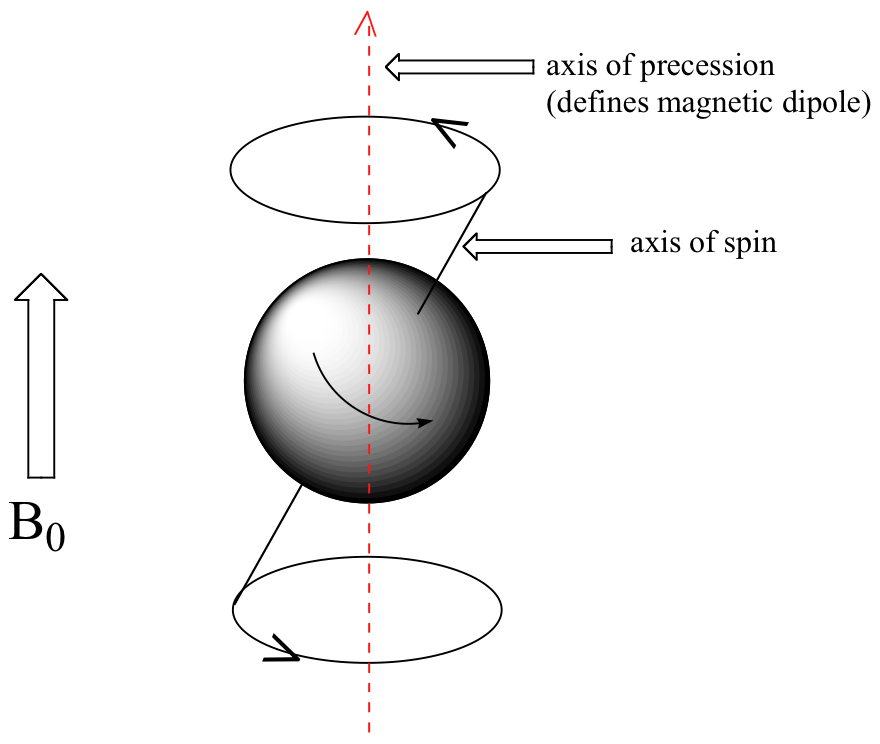
\includegraphics[]{fig/4-1.png}
        \caption{Larmor precession:图中的自旋矢量是平均值$\braket{\mathcal{S}}$}
    \end{figure}

    \subsubsection*{Stern–Gerlach实验}
    我们下面考虑非均匀磁场, 这时不仅力偶矩不为$0$, 所受的合力也不为$0$, 合力的公式为:
    \begin{equation}
        \label{eq:4.78}
        \mathbf{F}=\nabla\left(\mathbf{\mu}\cdot\mathbf{B}\right)
    \end{equation}
    这里计算梯度的时候把$\mathbf{\mu}$当作只与时间有关, 与空间无关的矢量\footnote{确实, 由于粒子的运动, 磁矩也应该看作是与位置有关, 但是如果看一下
    这个公式的推导过程, 我们会发现它是在\uwave{某一时刻}考虑偶极子附近磁场变化情况得出的, 所以实际上求梯度的时候$\mathbf{\mu}$不参与, 它与时间的依赖性, 造成了$\mathbf{F}$随时间的变化}。
    我们考虑所加磁场在$z$方向上有个偏差$(\alpha\ll 1)$:
    \[\mathbf{B}\sim\left(B_0+\alpha z\right)\hat{\mathbf{k}}\]
    显然, 根据$\nabla\cdot\mathbf{B}=0$, 磁场一定会在$x$方向也有个偏差:
    \[\mathbf{B}=-\alpha x \hat{\mathbf{i}}+\left(B_0+\alpha z\right)\hat{\mathbf{k}}\]
    根据\ref{eq:4.78}, 受力可以写成:
    \begin{equation}
        \mathbf{F}=\gamma\alpha\left(S_z\hat{\mathbf{k}}-S_x\hat{\mathbf{i}}\right)
    \end{equation}
    
    由于拉莫尔进动效应, $S_x$变化的很快(磁场还是$z$方向占主导作用), 所以可以认为$F_x$平均效果为$0$, 最终粒子受到$z$方向的作用力偏转, 而且与$S_z$成正比。
    
    实验观测到最终粒子被分为一系列离散的粒子流, 这也说明了粒子的自旋角动量的量子性(如果是连续的显然应该各个方向出射的粒子都有)。这个实验在量子态的测量和制备上也具有
    重大意义, 我们可以利用这个实验装置入射粒子流最终得到一系列的$S_z$取值不同的粒子, 这个过程是量子态的\textbf{制备}。我们还可以让一个粒子通过这个装置, 根据它出射的角度去确定
    其$S_z$的取值, 这便是量子态的\textbf{测量}。
    \begin{figure}[htbp]
        \centering
        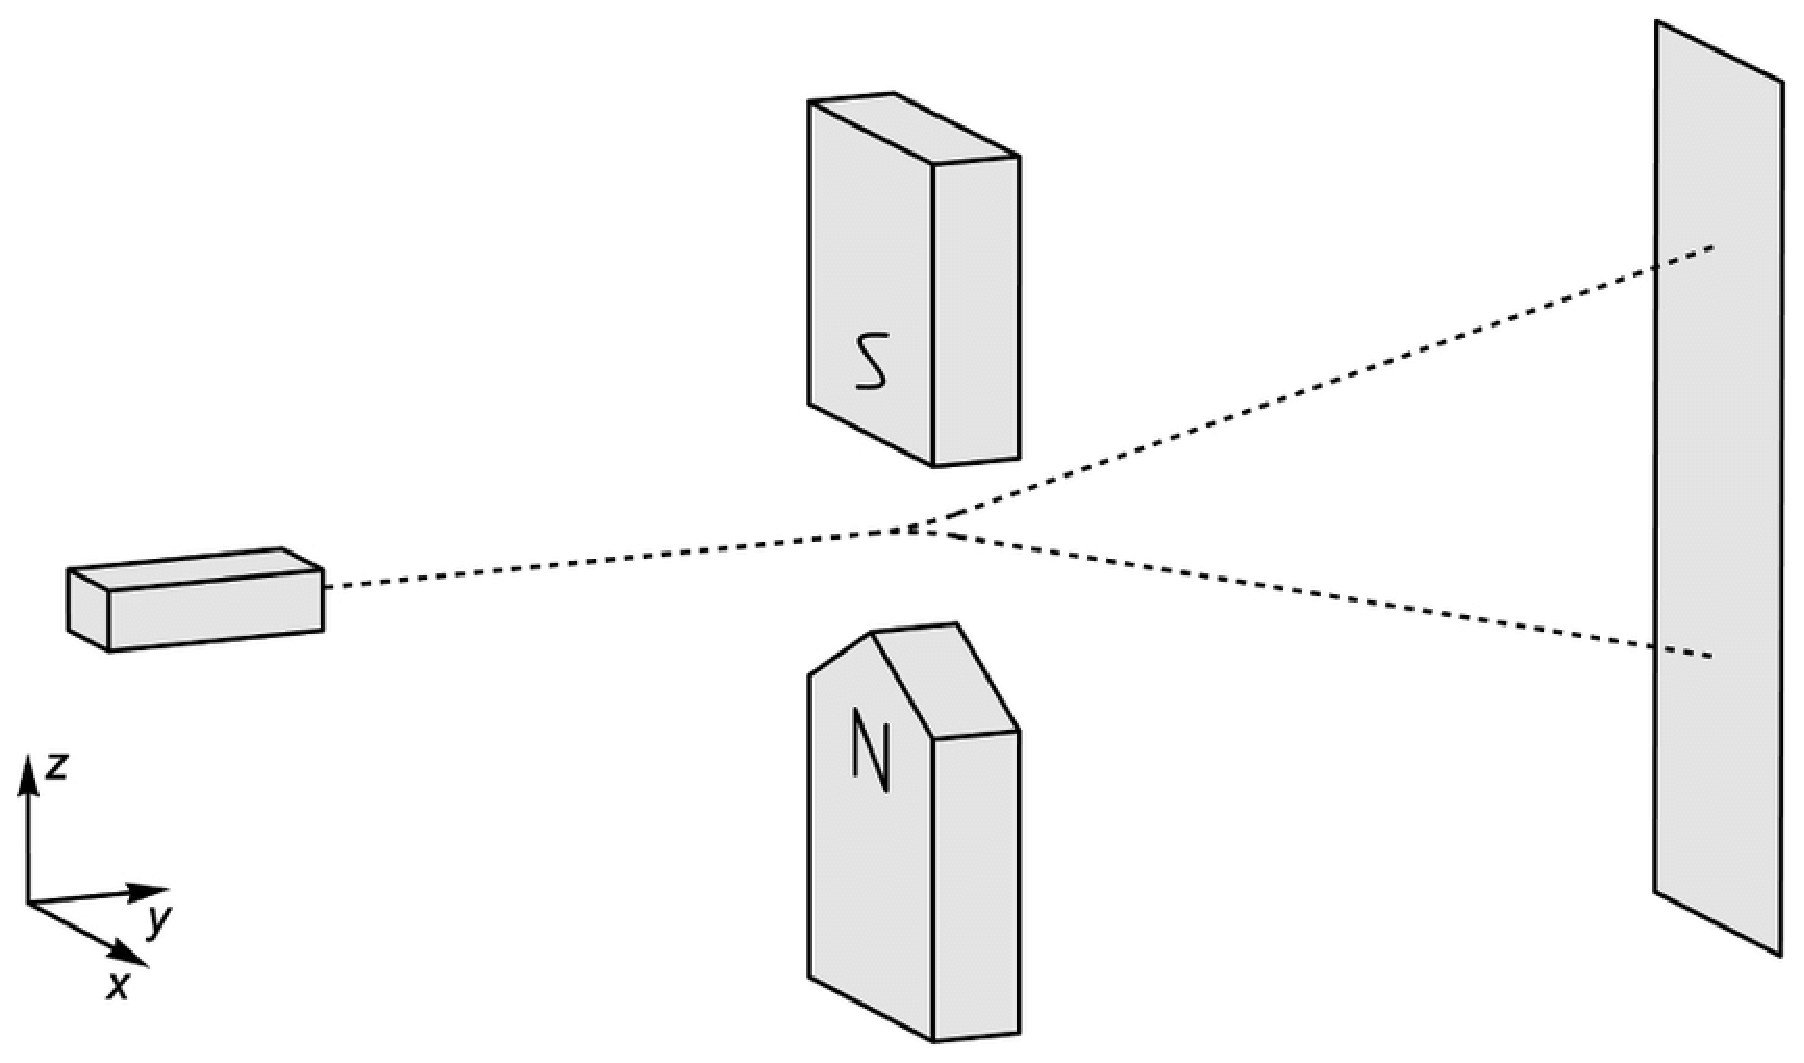
\includegraphics[scale=0.35]{fig/4-2.eps}
        \caption{The Stern–Gerlach apparatus:自旋向上的粒子向上偏转, 反之向下偏转}
    \end{figure}
    \section{数学准备:张量积}
    这一节主要是线性代数的补充附录, 其实这部分内容早该讲了, 因为从一维量子力学引入到三维是自然的, $\mathscr{E}_r\cong\mathscr{E}_x\otimes\mathscr{E}_y\otimes \mathscr{E}_z $。
    
    \begin{define}{张量积空间}
        张量积空间是两个向量空间通过运算“$\otimes$”生成的新的向量空间:
        \[\mathscr{E}=\mathscr{E}_1\otimes\mathscr{E}_2\]
        $\mathscr{E}$中的元素由$\mathscr{E}_1$和$\mathscr{E}_2$中元素的张量积构成\footnote{$\ket{\chi}\otimes\ket{\varphi}$和$\ket{\varphi}\otimes\ket{\chi}$是一样的。}:
        \[\forall\ket{\varphi}\in\mathscr{E}_1,\ket{\chi}\in\mathscr{E}_2\Rightarrow\ket{\varphi}\otimes\ket{\chi}\]
        其中张量积运算满足“双线性”:
        \begin{align}
            & \left[\lambda\ket{\varphi}\right]\otimes\ket{\chi}=\lambda\left[\ket{\varphi}\otimes\ket{\chi}\right]\\
            & \ket{\varphi}\otimes\left[\mu\ket{\chi}\right]=\mu\left[\ket{\varphi}\otimes\ket{\chi}\right]
        \end{align}
        \begin{align}
            & \ket{\varphi}\otimes\left[\ket{\chi_1}+\ket{\chi_2}\right]=\ket{\varphi}\otimes\ket{\chi_1}+\ket{\varphi}\otimes\ket{\chi_2}\\
            & \left[\ket{\varphi_1}+\ket{\varphi_2}\right]\otimes\ket{\chi}=\ket{\varphi_1}\otimes\ket{\chi}+\ket{\varphi_2}\otimes\ket{\chi}
        \end{align}
        而且如果$\{\ket{\varphi_i}\}$是$\mathscr{E}_1$中的一组基, $\{\ket{\chi_l}\}$是$\mathscr{E}_2$中的一组基。那么他们的张量积$\{\ket{\varphi_i}\otimes\ket{\chi_l}\}$
        构成了$\mathscr{E}$中的一组基。
    \end{define}
    \subsection*{$\mathscr{E}$中的内积}
    张量积空间中内积的定义依赖于$\mathscr{E}_1,\mathscr{E}_2$中标量积的定义。首先我们换一个更加清爽的符号记$\mathscr{E}$中的向量:
    \[\ket{\varphi\chi}\equiv\ket{\varphi}\otimes\ket{\chi}\]
    下式给出了内积的定义:
    \begin{equation}
        \boxed{
            \Braket{\varphi_2\chi_2|\varphi_1\chi_1}\equiv\Braket{\varphi_2|\varphi_1}\Braket{\chi_2|\chi_1}
        }
    \end{equation}
    根据这个定义我们可以立即得出, 如果我们得到了两个空间中的正交归一基, 那么对应的张量积在张量积空间中构成的基底也是正交归一的, 只是这个时候要使用两个指标来标记:
    \[\Braket{\varphi_{i^\prime}\chi_{l^\prime}|\varphi_i\chi_l}=\delta_{ii^\prime}\delta_{ll^\prime}\]
    \subsection*{算符的张量积}
    设$\hat{A}$是定义在$\mathscr{E}_1$上的一个算符, $\hat{B}$定义在$\mathscr{E}_2$上, 它们的延伸算符按照下式定义:
    \[\tilde{A}\left[\ket{\varphi}\otimes\ket{\chi}\right]=\left[\tilde{A}\ket{\varphi}\right]\otimes\ket{\chi}
    ,\tilde{B}\left[\ket{\varphi}\otimes\ket{\chi}\right]=\ket{\varphi}\otimes\left[\tilde{B}\ket{\chi}\right]\]
   
    按照上面的定义可以得出:\[\left[\tilde{A},\tilde{B}\right]=0\]这实际上就是在说, 两个无相互作用的粒子构成的体系, 它们两个之间的任意力学量都是对易相容的, 也
    就是说一定可以同时精确确定两个粒子的任意力学量。\footnote{当然, 这是非常自然的, 除非两个粒子之间建立了纠缠态, 否则我测量一个粒子肯定不会干扰到另一个粒子的测量, 但是我单独测量一个粒子, 根据不确定性原理, 测量是会干扰体系影响下一次测量的。}

    算符$A,B$的张量积定义为:
    \begin{equation}
        \boxed{
            \hat{A}\otimes\hat{B}\equiv\tilde{A}\tilde{B}
        }
    \end{equation}
    或直接写为:
    \begin{equation}
        \left(\hat{A}\otimes\hat{B}\right)\ket{\varphi\chi}=\left[\hat{A}\ket{\varphi}\right]\otimes\left[\hat{B}\ket{\chi}\right]
    \end{equation}
    
    例如, 按照这个定义, $\mathscr{E}$中的投影算符可以写为:
    \begin{equation}
        \ket{\varphi\chi}\bra{\varphi\chi}=\left(\ket{\varphi}\bra{\varphi}\right)\otimes\left(\ket{\chi}\bra{\chi}\right)
    \end{equation}
    \subsection*{符号约定}
    量子力学中, 我们的符号体系尽量简化, 但是有时候会存在含糊不清的情况, 这个时候就要根据上下文来判断了, 具体简化如下:
    \begin{itemize}
        \item $\ket{\varphi}\otimes\ket{\chi}\Rightarrow\ket{\varphi}\ket{\chi}$
        \item $\hat A\otimes \hat B\Rightarrow \hat{A}\hat{B}$
        \item $\tilde{A}\Rightarrow\hat{A}$
    \end{itemize}
    
    一般来说, 只要根据上下文确定算符的作用对象, 就不会有含糊的地方, 而且这里的符号简化在物理上也很自然。我们这里只是简要的介绍了一下多重线性代数的一些定义, 不过
    对于下一节要讲的内容来说已经够用了。

    \section{角动量的合成}
    这一部分的内容还是比较深奥的, 我们只是用初等的方法做一个极其简单的介绍。

    我们下面考虑两个自旋耦合的粒子体系, 我们只考虑它们的自旋。 单个粒子的态空间为$\mathscr{E}_1$和$\mathscr{E}_2$。 以第一个粒子为例, 在自旋态空间中, $\mathcal{S}^2, \mathcal{S}_z$
    构成了一个CSCO, 所以我们可以使用它们的本征值所对应的参数$s_1,m_1$, 去完整描述这单个粒子, 而且它们的共同本征矢$\ket{s_1,m_1}$构成了$\mathscr{E}_1$中的基底。对于某个粒子来说, 其自旋角量子数$s$
    是不会变的, 所以实际上我们只需要$m_1$这一个参数就可以完整描述一个$s_1$已知的粒子的自旋态。
    
    两个粒子耦合的自旋态空间$\mathscr{E}$是两个粒子自身的自旋态空间的张量积, 且对应的基底可以用下式确定:
    \[\ket{s_1,s_2,m_1,m_2}=\ket{s_1,m_1}\otimes\ket{s_2,m_2}\]
    显然$s_1,s_2,m_1,m_2$四个参数加上态之间的线性组合完全描绘了整个系统, 实际上是因为${\mathcal{S}_1}^2$,\\${\mathcal{S}_2}^2$,$\mathcal{S}_{1z}$,$\mathcal{S}_{2z}$在$\mathscr{E}$中构成了一个CSCO,
    由于$s_1,s_2$又是固定的, 所以实际上只需要$m_1,m_2$就可以描绘整个系统。当然我们也可以找其它的CSCO, 用别的参数去描述这个系统, 但是总的自由度就是$4$\footnote{当然, 如果你不算$s_1,s_2$的话就是$2$}。

    可以证明总的自旋角动量算符和其$z$轴上的分量算符\footnote{下面的推导中我们使用上一节的符号约定, 略去延伸算符的$\tilde{}$}与${\mathcal{S}_1}^2,{\mathcal{S}_2}^2$一起构成了一个CSCO:
    \begin{align}
        &\mathcal{S}^2=\left(\mathcal{S}_1+\mathcal{S}_2\right)^2={\mathcal{S}_1}^2+{\mathcal{S}_2}^2+2\mathcal{S}_1\cdot\mathcal{S}_2\\
        &\mathcal{S}_z=\mathcal{S}_{1z}+\mathcal{S}_{2z}
    \end{align}
    上式中利用了$\left[\mathcal{S}_1,\mathcal{S}_2\right]=0$, 而且:
    \[\mathcal{S}_1\cdot\mathcal{S}_2\equiv\mathcal{S}_{1x}\mathcal{S}_{2x}+\mathcal{S}_{1y}\mathcal{S}_{2y}+\mathcal{S}_{1z}\mathcal{S}_{2z}\]
    
    那么根据代数结构上的类似性我们就可以考虑使用$\mathcal{S}^2$和$\mathcal{S}_z$对应的联系本征值的参数$s,m$以及其共同本征矢$\ket{s,m}$去描绘整个系统。且类似的去定义本征值和$s,m$之间的关系:
    \begin{align}
        &\mathcal{S}^2\ket{s,m}=\hbar^2s(s+1)\ket{s,m}\\
        &\mathcal{S}_z\ket{s,m}=\hbar m\ket{s,m}    
    \end{align}
    
    这也就是我们要做的事情, 把两个自旋等效为一个自旋, 并且写出对应的自旋量子数。对于一个粒子而言,$s$是确定的, 但是对于两个粒子构成的体系来说, 就不一定了, $s$的取值受$m_1,m_2$的影响, 所以现在正是要去求出所有的本征值和本征矢。
    这个问题很复杂, 我们下面在两个自旋$\frac{1}{2}$的粒子体系中具体考虑这个问题, 用的也是初等的方法。

    \subsection*{双自旋$\frac{1}{2}$体系}
    根据$\mathcal{S}$的定义可以证明它也具有\ref{eq:4.48}所示的代数结构, 所以我们也类似定义$\mathcal{S_\pm}$, $\mathcal{S}$与$\mathcal{S}_z$的共同本征矢$\ket{s,m}$也应该
    满足\ref{eq:4.60}。

    如果我们考虑使用$m_1,m_2$去描述系统, 那么很容易得出系统的一组基底:
    \begin{equation}
        \label{eq:4.92}
        \begin{split}
            &\ket{\uparrow\uparrow}=\ket{\frac{1}{2},\frac{1}{2},\frac{1}{2},\frac{1}{2}}\\
            &\ket{\uparrow\downarrow}=\ket{\frac{1}{2},\frac{1}{2},\frac{1}{2},-\frac{1}{2}}\\
            &\ket{\downarrow\uparrow}=\ket{\frac{1}{2},\frac{1}{2},-\frac{1}{2},\frac{1}{2}}\\
            &\ket{\downarrow\downarrow}=\ket{\frac{1}{2},\frac{1}{2},-\frac{1}{2},-\frac{1}{2}}
        \end{split}
    \end{equation}
    实际上就是$\{\ket{\uparrow},\ket{\downarrow}\}\otimes\{\ket{\uparrow},\ket{\downarrow}\}$。而且这些本征矢同时也是$\mathcal{S}_z$的本征矢:
    \begin{align*}
        &\mathcal{S}_z\ket{\uparrow\uparrow}=+\ket{\uparrow\uparrow}&m&=1\\
        &\mathcal{S}_z\ket{\uparrow\downarrow}=0&m&=0\\
        &\mathcal{S}_z\ket{\downarrow\uparrow}=0&m&=0\\
        &\mathcal{S}_z\ket{\downarrow\downarrow}=-\ket{\downarrow\downarrow} &m&=-1
    \end{align*}
   
    但是这些本征矢却不全是$\mathcal{S}^2$的本征矢, 下面的方法具有猜测性, 根据对于某个自旋有:
    \[\mathcal{S}_-\ket{\uparrow}=\hbar\ket{\uparrow}\quad\mathcal{S}_-\ket{\downarrow}=0\]
    可以得到:
    \begin{align*}
        \mathcal{S}_-\ket{\uparrow\uparrow}&=\hbar\left(\ket{\downarrow\uparrow}+\ket{\uparrow\downarrow}\right)\\
        &=\hbar\sqrt{2}\cdot\frac{1}{\sqrt{2}}\left(\ket{\downarrow\uparrow}+\ket{\uparrow\downarrow}\right)
    \end{align*}
    通过上式的第二步变形, 后面的叠加态满足了归一化原理, 我们再次对其作用降阶算符:
    \[\mathcal{S}_-\left[\frac{1}{\sqrt{2}}\left(\ket{\downarrow\uparrow}+\ket{\uparrow\downarrow}\right)\right]=\hbar\sqrt{2}\ket{\downarrow\downarrow}\]
    上面得到的态再次降阶就变成$0$了。

    通过上面的铺垫我们下面的说法也显得比较自然了。如果$\ket{\uparrow\uparrow}$是$\mathcal{S}^2$和$\mathcal{S}_z$的共同本征矢, 那么显然$m=1$, 再根据\ref{eq:4.60}
    和文中出现的$\sqrt{2}$, 以及$m=-1,0,1$的取值。种种迹象表明$s$应该等于$1$, 而且按照这个想法, $\mathcal{S}_-$每次操作确实是降低了$m$的值。
    \begin{equation}
        \boxed{
            \left\{
                \begin{matrix}
                   &\ket{1,1}=\ket{\uparrow\uparrow}\\
                    &\ket{1,0}=\frac{1}{\sqrt{2}}\left(\ket{\downarrow\uparrow}+\ket{\uparrow\downarrow}\right)\\
                    &\ket{1,-1}=\ket{\uparrow\uparrow} 
                \end{matrix}
            \right\}s=1\text{(triplet)}
        }
    \end{equation}
    而且\ref{eq:4.92}中$m=0$的$\mathcal{S}_z$简并的情况应该是对应了$s=0$的另一种取值:
    \begin{equation}
        \boxed{
            \left\{\ket{0,0}=\frac{1}{\sqrt{2}}\left(\ket{\uparrow\downarrow}-\ket{\downarrow\uparrow}\right)\right\}\quad s=0\text{(singlet)}
        }
    \end{equation}

    当然, 目前为止我们都只能说是把结果\uwave{猜}出来了, 还应该进一步去证明。 其实, 只要利用$\mathcal{S}^2$的定义, 是很好证明上面的三重态和单重态分别对应其本征值$2\hbar$和$0$的
    本征矢\footnote{后面会专门规范一下\uwave{矢量算符}的符号问题}:
    \[\mathcal{S}^2={\mathcal{S}_1}^2+{\mathcal{S}_2}^2+2\mathcal{S}_1\cdot\mathcal{S}_2\]
    

    事实上, 对于一般的系统, 可以证明$s$的取值为:
    \begin{equation}
        \boxed{s=(s_1+s_2),(s_1+s_2-1),\ldots,|s_1-s_2|}
    \end{equation}
    
    当然, $m$的取值问题就非常trival了, 直接相加就好了, 并且也会从$-s$取到$s$。而且$\ket{s,m}$(耦合表象)和$\ket{s_1,s_2,m_1,m_2}$(非耦合表象)这两种表象之间有如下的变换关系:
    \begin{equation}
        \ket{s,m}=\sum_{m_1+m_2=m}C_{m_1m_2m}^{s_1s_2s}\ket{s_1,s_2,m_1,m_2}
    \end{equation}
    其中$C_{m_1m_2m}^{s_1s_2s}$是\textbf{CG系数}\footnote{Clebsch–Gordan coefficients}。利用这个式子, 我们可以根据$s$和$m$的取值推断出测量体系中的单个粒子得到结果的概率分布。
    反过来, 也可以已知单个粒子的状态参量, 根据下面的式子使用$\ket{s,m}$表出, 从而计算出测量结果$s,m$的取值和概率分布:
    \begin{equation}
        \ket{s_1,s_2,m_1,m_2}=\sum_{m}C_{m_1m_2m}^{s_1s_2s}\ket{s,m}\quad (m=m_1+m_2)
    \end{equation}
    
    这一切的一切都需要使用$CG$系数表, 其使用方法从书上的具体例子和习题中去领会。
    
    最后, 我们这里虽然只考虑了两个自旋的叠加, 但实际上轨道角动量和自旋也是能如此操作的, 一样的套路, 把其中一个$s_1$(或者$s_2$)换成$\ell$就可以了, 因为就从代数结构上来说, 自旋和轨道角动量没啥差别, 
    要说差别只能说一个的本征矢只能使用狄拉克符号表示, 无法在位置表象下表示为波函数。
    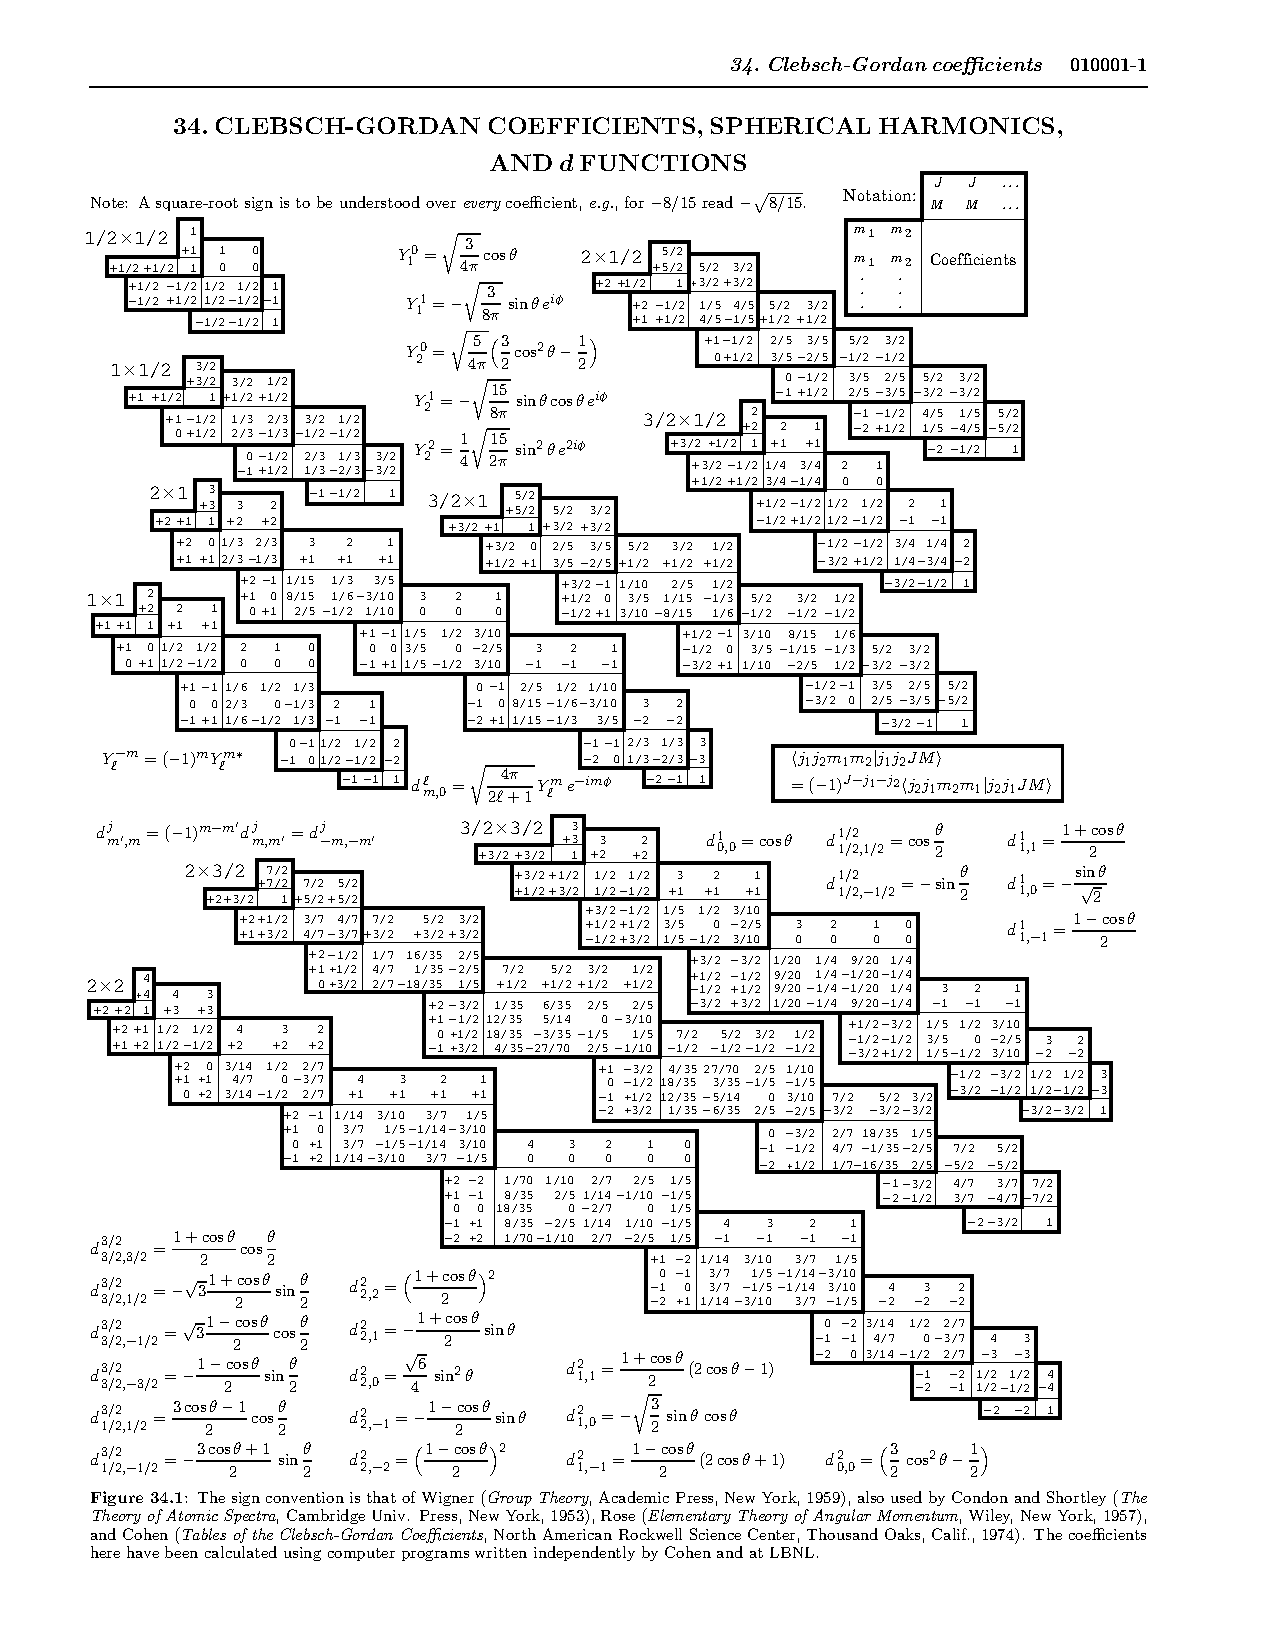
\includepdf{fig/CG-coefficients.pdf}
    \newpage
    \subsection*{$\vec{R}$到底表示什么?}
    我们前面写的$\vec{R},\vec{P},\vec{L},\ldots$这些算符实际上都应该看成是三个算符的缩并记法。这样的话我们可以大大简化我们的记号, 比如三个对易式:
    \begin{equation}
        \left[L^2,L_x\right]=\left[L^2,L_y\right]=\left[L^2,L_z\right]=0
    \end{equation}
    可以简单的记为:
    \begin{equation}
        \left[L^2,\vec{L}\right]=0
    \end{equation}

    你显然不能直接把这样记录的算符直接作用在波函数上, 因为$\vec{R}\Psi$你要认为是三个分量算符$X,Y,Z$分别作用在$\Psi$上, 这样得到的就不是$L^2$中的波函数了, 而是
    三个波函数构成的一个向量。
    
    但是使用这个记号要非常小心, 因为每个这样的式子都表示了三个分量式子, 特别是缩写的对易子, 下面的对易子是有意义的:
    \begin{equation}
        \label{eq:4.100}
        \left[\frac{P^2}{2m},\vec{R}\right]=
    \end{equation}
    
    因为$P^2$解释为$P_x^2+P_y^2+P_z^2$, 上面的式子根据$R$的下标来标记,等价于三个分量式。使用这种矢量形式记的式子可以很大程度上方便我们的形式计算, 比如:
    \begin{align*}
        \left(\vec{P}-q\vec{A}\right)^2 f&= \left(\vec{P}-q\vec{A}\right)\cdot\left(\vec{P}-q\vec{A}\right)f\\
        &=\left(P^2+q^2A^2-q\vec{P}\cdot\vec{A}-q\vec{A}\cdot \vec{P}\right)f\\
        &=-\hbar^2\nabla^2 f+q^2A^2f+i\hbar q\vec{A}\cdot\nabla f+i\hbar qf\nabla \cdot\vec{A}+i\hbar q\vec{A}\cdot \nabla f\\
        &=\left(-\hbar^2\nabla^2+2i\hbar q\vec{A}\cdot\nabla\right) \quad (\text{利用规范变换我们取:}\nabla\cdot \vec{A}=0)
    \end{align*}
    对的, 形式上和矢量的运算法则是一样的!基本上你形式上这样算不会出现差错。但是一旦涉及到对易子的计算就要格外小心了, 比如:
    \[
        \left[\left(\vec{P}-q\vec{A}\right)^2,\vec{P}-q\vec{A}\right]
    \]
    
    你不能想当然的就认为是$\left[f(\hat{A}),\hat{A}\right]$形式, 觉得它就是$0$。实际上你在考虑这个运算时, 应当先把这个式子分解为三个分量式, 分别考虑, 最后再看能不能写成合并的形式。
    而不是只想着一步到位。
    
    再比如计算\ref{eq:4.100}的时候你也不能使用公式把它拆开成下面的式子去计算:
    \[\vec{P}\left[\frac{\vec{P}}{2m},\vec{R}\right]+\left[\frac{\vec{P}}{2m},\vec{R}\right]\vec{P}\]
    
    因为我们碰到的对易子形式上看都是[scalar,vector]的形式, 但是$[\vec{P},\vec{R}]$是[vector,vector]的形式。如果你硬是想搞一个良好的定义的话
    需要涉及到$3\times 3$个指标, 而且这种缩并的记号每个都不是代表单独的一个算符, 它们之间的算符复合乘法运算已经失去了意义, 也不能想当然的直接把$[\vec{P},\vec{R}]$
    用对易子的定义拆开来算。总之, 遇到这种记号就回到分量形式去看, 也不需要复杂地定义一套对于这套记号的专属对易子运算法则。只要清楚$P^2$这种平方的算符记号代表什么就可以消除很多疑惑了。


    \section{电磁相互作用}
    本节我们讨论一下在电磁场的作用下, 带电粒子的量子行为, 前面已经对有自旋粒子做了部分修正, 下面的考虑都是无自旋粒子的动力学, 经典情况已经由麦克斯韦方程加洛伦兹力公式
    完全描述了。但是当我们考虑量子力学的时候会有意想不到的事情发生。

    \subsection*{最小电磁耦合原理}
    矢量力学中对电磁作用动力学的描述是洛伦兹力公式:
    \begin{equation}
        \mathbf{F}=q\left(\mathbf{E}+\mathbf{v}\times\mathbf{B}\right)
    \end{equation}
    哈密顿力学版本:
    \begin{equation}
        \label{eq:4.102}
        H=\frac{1}{2m}\left(\mathbf{p}-q\mathbf{A}\right)^2+q\varphi
    \end{equation}
    其中:
    \begin{equation}
        \mathbf{E}=-\nabla\varphi-\frac{\partial\mathbf{A}}{\partial t},\mathbf{B}=\nabla\times \mathbf{A}
    \end{equation}
    我们直接将\ref{eq:4.102}中的力学量换成算符得到哈密顿算符:
    \begin{equation}
        \hat{H}=\frac{1}{2m}\left(-i\hbar\nabla-q\mathbf{A}\right)^2+q\varphi
    \end{equation}
    故薛定谔方程在电磁作用下变成了:
    \begin{equation}
        \label{eq:4.105}
        \boxed{
            i\hbar\frac{\partial\Psi}{\partial t}=\left[\frac{1}{2m}\left(-i\hbar\nabla-q\mathbf{A}\right)^2+q\varphi\right]\Psi
        }
    \end{equation}
    \subsection*{规范不变性}
    我们对$A$和$\varphi$施以下面的变换:
    \begin{equation}
        \mathbf{A}\rightarrow\mathbf{A}+\nabla\Lambda,\varphi\rightarrow\varphi-\frac{\partial\Lambda}{\partial t}
    \end{equation}
    
    其中$\Lambda$是一个任意的关于时间和空间的函数。我们称之为\textbf{规范变换}, 而且很容易证明在这个变换下$E$和$B$具有不变性。这也说明了$A$和$\varphi$是没有绝对意义的, 就像势能一定要先选取势能点一样, 它们也是有多种形式的。
    一般我们选取$\nabla\cdot\mathbf{A}=0$。

    在这个变换下, 薛定谔方程\ref{eq:4.105}变成了:
    \begin{equation}
        \label{eq:4.107}
        i\hbar\frac{\partial\Psi^\prime}{\partial t}=\left[\frac{1}{2m}\left(-i\hbar\nabla-q\mathbf{A}^\prime\right)^2+q\varphi^\prime\right]\Psi^\prime
    \end{equation}
    下面我们来证明, 这个变换只是让解多出了一个指数因子:
    \begin{equation}
        \label{eq:4.108}
        \Psi^\prime=e^{iq\Lambda/\hbar}\Psi
    \end{equation}

    而我们知道这样的两个解在物理上是不可区分的, 也就是说虽然薛定谔方程是直接与矢势相关联的, 但是矢势的选取不同, 也就是做规范变换, 并不会对解造成任何影响。所以薛定谔方程
    具有\textbf{规范不变性}。
    \begin{thinknote}
        Proof:

        \setlength\parindent{2em}我们的证明是验证性证明, 依据\ref{eq:4.108}先去计算\ref{eq:4.107}的左边:
        \begin{align*}
            i\hbar\frac{\partial\Psi^\prime}{\partial t}&=i\hbar\left[e^{iq\Lambda/\hbar}\frac{\partial\Psi}{\partial t}+\frac{i q}{\hbar}\frac{\partial\Lambda}{\partial t}e^{iq\Lambda/\hbar}\Psi\right]\\
            &=e^{iq\Lambda/\hbar}\left[\frac{1}{2m}\left(-i\hbar\nabla-q\mathbf{A}\right)^2+q\varphi-q\frac{\partial\Lambda}{\partial t}\right]\Psi
        \end{align*}
        上面最后一步代入了\ref{eq:4.105}。下面代入规范变换得:
        \begin{equation}
            i\hbar\frac{\partial\Psi^\prime}{\partial t}=e^{iq\Lambda/\hbar}\left[\frac{1}{2m}\left(-i\hbar\nabla-q\mathbf{A}^\prime+q\nabla\Lambda\right)^2+q\varphi\right]\Psi
        \end{equation}
        看来我们要做的就是将$e^{iq\Lambda/\hbar}$移到$\Psi$那里去。首先注意到:
        \begin{equation}
            i\hbar\nabla\left(e^{iq\Lambda/\hbar} f\right)=-i\hbar e^{iq\Lambda/\hbar}\nabla f+q\left(\nabla\Lambda\right)e^{iq\Lambda/\hbar}f=e^{iq\Lambda/\hbar}\left[i\hbar\nabla+q\nabla\Lambda\right]f
        \end{equation}
        其中$f$是任意的一个函数。所以我们立刻得到:
        \[e^{i q \Lambda / \hbar}\left[-i \hbar \nabla-q \mathbf{A}^{\prime}+q(\boldsymbol{\nabla} \Lambda)\right] f=\left(-i \hbar \nabla-q \mathbf{A}^{\prime}\right)\left(e^{i q \Lambda / \hbar} f\right)\]
        最后:
        \begin{equation}
            \begin{aligned}
            &e^{i q \Lambda / \hbar}\left[-i \hbar \nabla-q \mathbf{A}^{\prime}+q(\boldsymbol{\nabla} \Lambda)\right]^{2} \Psi\\ &=e^{i q \Lambda / \hbar}\left[-i \hbar \boldsymbol{\nabla}-q \mathbf{A}^{\prime}+q(\boldsymbol{\nabla} \Lambda)\right] \underbrace{e^{-i q \Lambda / \hbar} e^{i q \Lambda / \hbar}\left[-i \hbar \nabla-q \mathbf{A}^{\prime}+q(\boldsymbol{\nabla} \Lambda)\right] \Psi}_{f} \\
            &=\left(-i \hbar \boldsymbol{\nabla}-q \mathbf{A}^{\prime}\right)\left[e^{i q \Lambda / \hbar} e^{-i q \Lambda / \hbar}\left(-i \hbar \nabla-q \mathbf{A}^{\prime}\right)\left(e^{i q \Lambda / \hbar} \Psi\right)\right] \\
            &=\left(-i \hbar \boldsymbol{\nabla}-q \mathbf{A}^{\prime}\right)^{2} \Psi^{\prime} .
        \end{aligned}
        \end{equation}
        即:
        \begin{equation}
            i \hbar \frac{\partial \Psi^{\prime}}{\partial t}=\left[\frac{1}{2 m}\left(-i \hbar \nabla-q \mathbf{A}^{\prime}\right)^{2}+q \varphi^{\prime}\right] \Psi^{\prime}
        \end{equation}
        \hfill $\square$\par
    \end{thinknote}
    
    在电动力学中, 我们引入矢势很大程度上是为了数学上的便利。但是在量子力学中, 矢势往往较与经典理论有更大的物理意义, 当然, 它们虽然会导致一些物理上和经典力学有很大
    不同的可观测效应, 但是它们本省仍旧是不可测量的, 否则它们将是绝对的, 量子力学就不再是规范对称了。这里有个很有趣的例子就是下面要讲的A-B效应, 因为它说明了即使某处并没有
    磁场和电场, 只要$\mathbf{A}\neq 0$, 在量子尺度上就会产生电磁作用的可观测效应。颠覆了很长一段时间科学界的认识, 之前认为发生电磁相互作用必须要有电场和磁场, 现在看来未必如此。 
    
    \subsection*{Aharonov-Bohm效应}
    这里我们只是粗略的介绍, 初步定性了解。

    考虑一根不带电无限长螺线管, 半径为$a$, 通入稳恒电流$I$, 外部电场和磁场都为$0$, 只有内部有磁场, 且磁通量为$\Phi$。虽然螺线管外部没有电磁场, 但是矢势不为$0$, 且可以得出:
    \[\mathbf{A}=\frac{\Phi}{2\pi r}\hat\phi(r>a)\]
    这里我们取的是柱坐标, $\hat{\phi}$是方位角方向单位矢量。
    \begin{figure}[htbp]
        \centering
        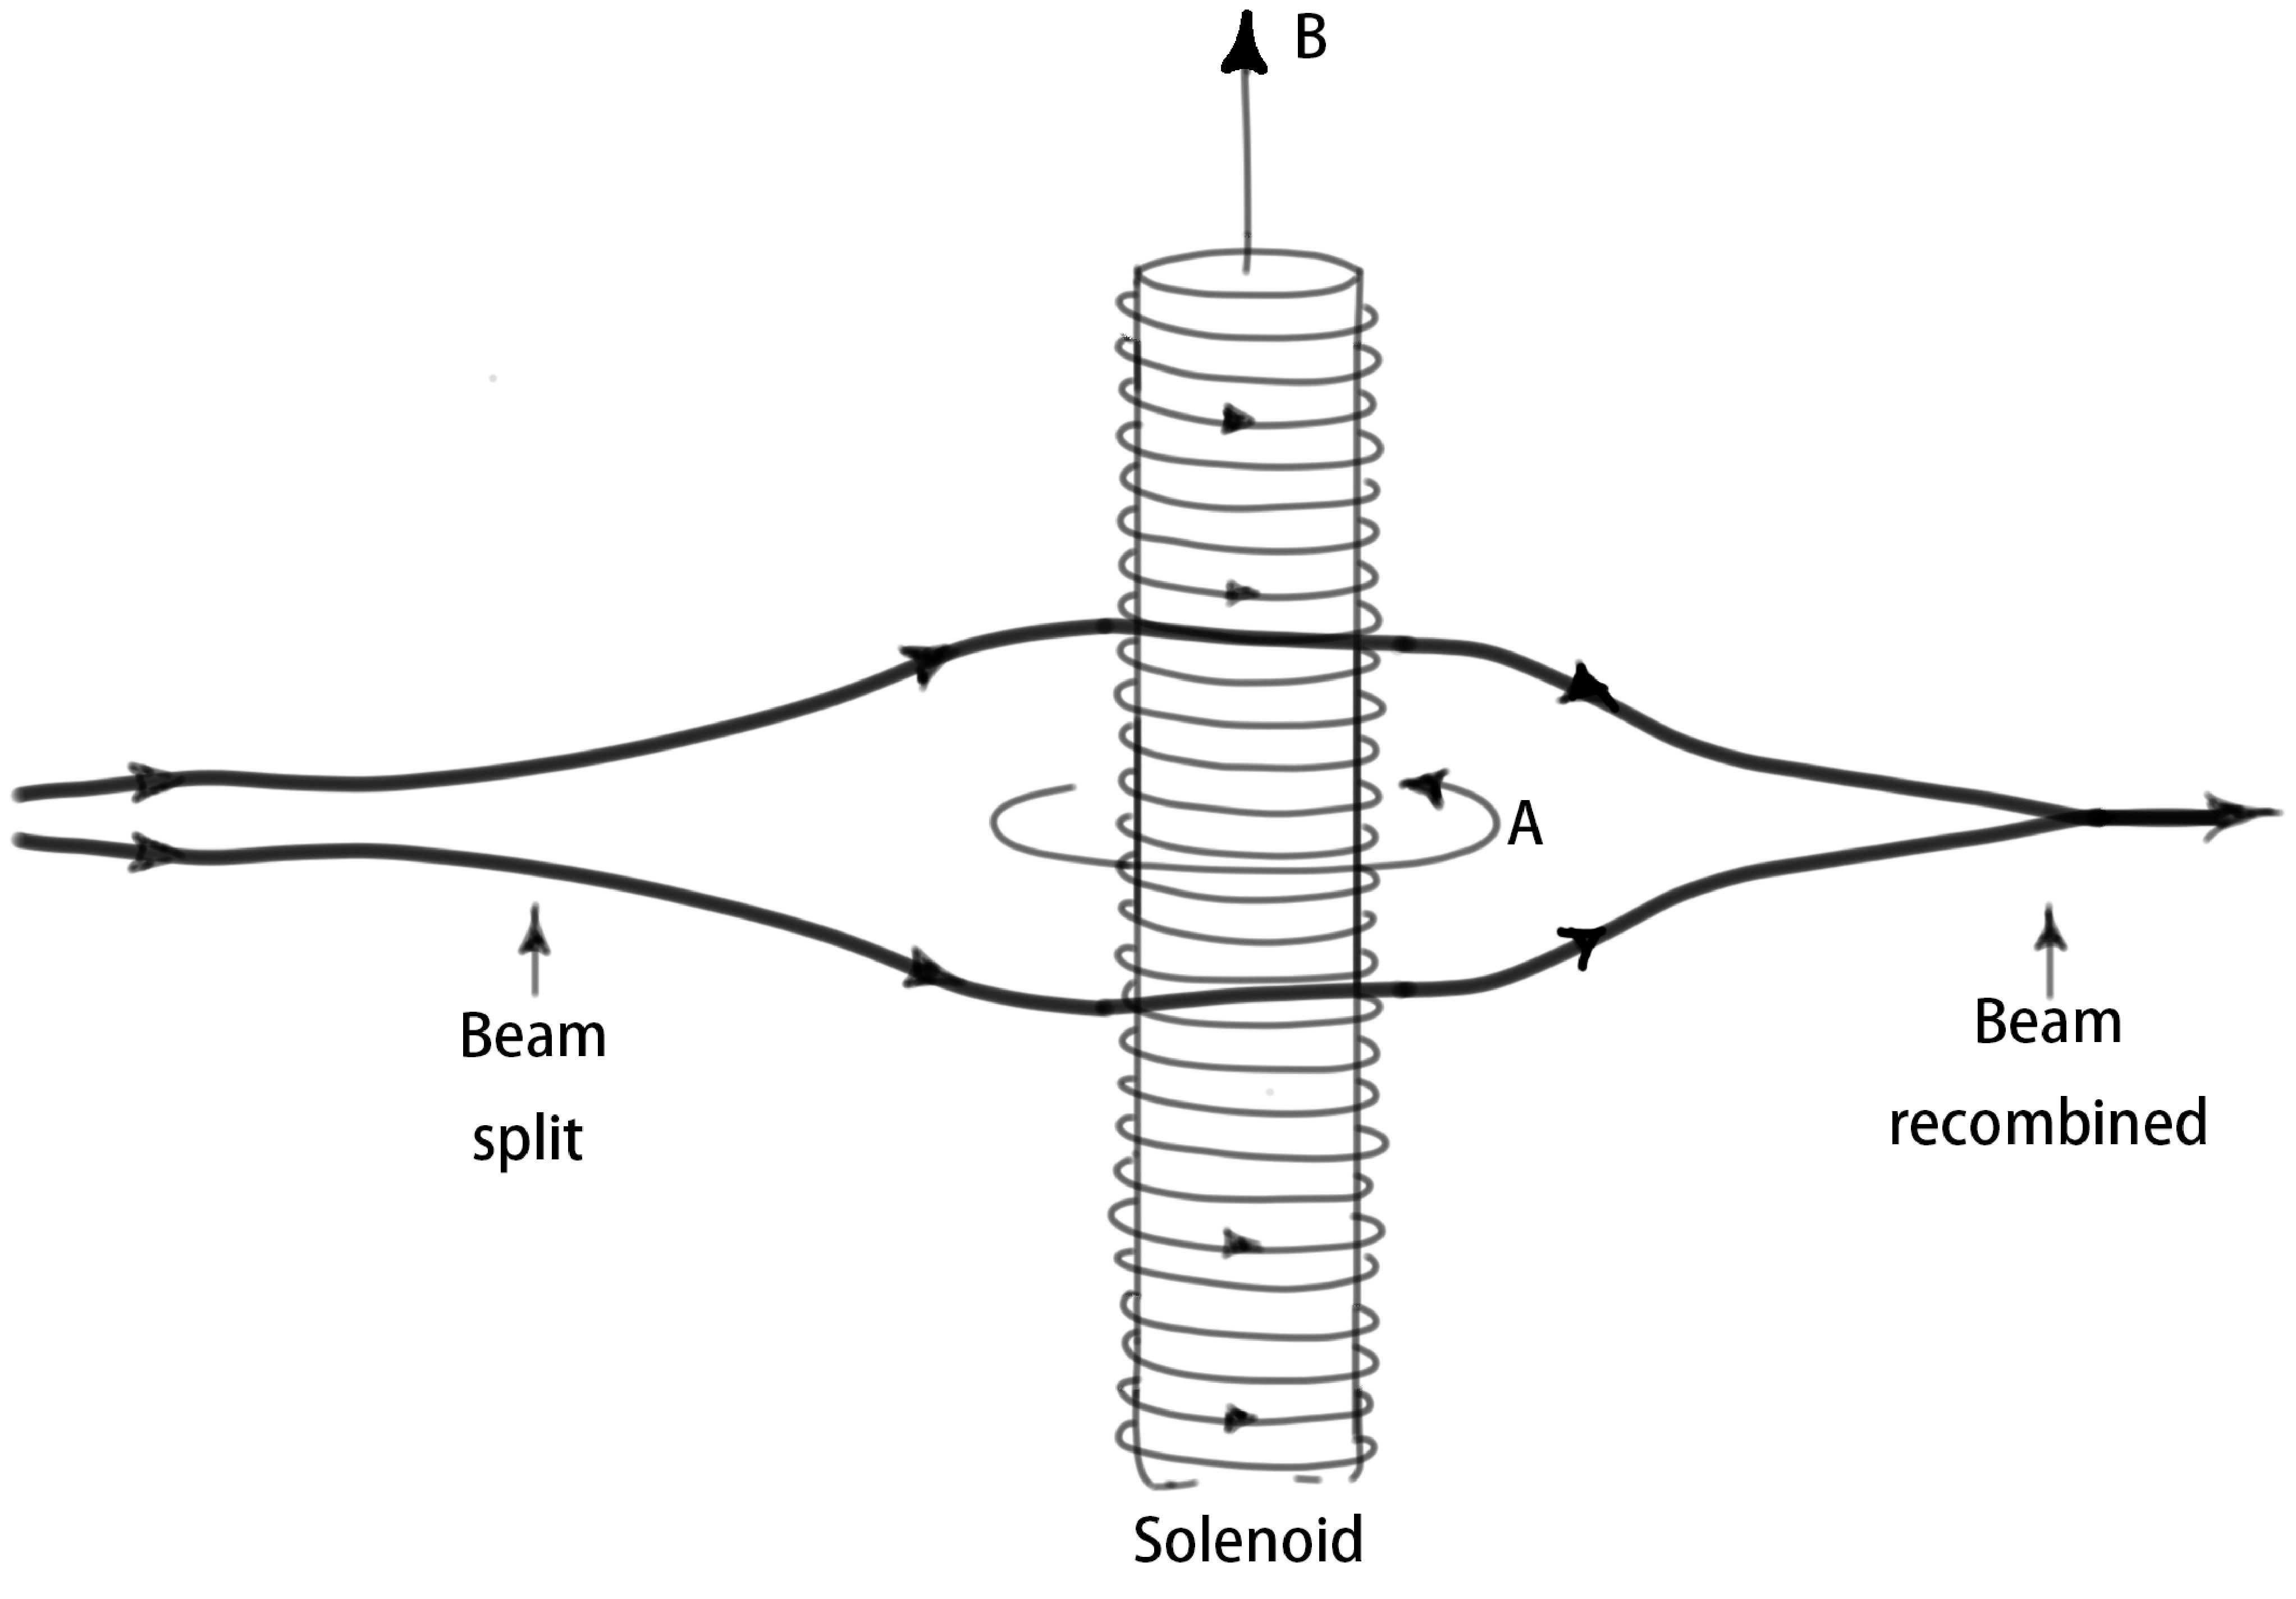
\includegraphics[scale=0.1]{fig/4-3.eps}
        \caption{AB效应}
        \label{AB效应}
    \end{figure}
    由于没有电场, 所以$\varphi=0$, 我们来具体考虑螺线管外部粒子的波函数, 薛定谔方程为:
    \[\left[\frac{1}{2 m}(-i \hbar \nabla-q \mathbf{A})^{2}\right] \Psi=i \hbar \frac{\partial \Psi}{\partial t}\]
    我们做如下换元:
    \[\Psi=e^{ig}\Psi^\prime\]
    其中$g(\mathbf{r})$定义为:
    \begin{equation}
        \label{eq:4.113}
        g(\mathbf{r})\equiv\frac{q}{\hbar}\int_\mathcal{O}^\mathbf{r}\mathbf{A}(\mathbf{r}^\prime)\cdot d\mathbf{r}^\prime
    \end{equation}
    
    上面的定义要求积分是与路径无关的, $\mathcal{O}$是任选的一个参考点, 显然这里的$\mathbf{A}$满足这些条件。注意到\footnote{注意下面的式子是$d\mathbf{r}$不是$\Delta\mathbf{r}$, 所以隐含了一个取极限的过程, 高阶项直接扔掉, 只保留一阶项, 而且是严格等于。}:
    \begin{align*}
        \nabla g\cdot d\mathbf{r}&=g(\mathbf{r}+d\mathbf{r})-g(\mathbf{r})\\
        &=\frac{q}{\hbar}\int_{\mathbf{r}}^{\mathbf{r}+d\mathbf{r}}\mathbf{A}(\mathbf{r}^\prime)\cdot d\mathbf{r}^\prime\\
        &=\frac{q}{\hbar}\mathbf{A}\cdot d\mathbf{r}
    \end{align*}
    故$ \nabla g=\frac{q}{\hbar}\mathbf{A}$, 代入$\nabla \Psi$表达式得到:
    \[(-i \hbar \nabla-q \mathbf{A}) \Psi=-i \hbar e^{i g} \nabla \Psi^\prime\]
    进一步运算得到:
    \[(-i \hbar \nabla-q \mathbf{A})^{2} \Psi=-\hbar^{2} e^{i g} \nabla^{2} \Psi^{\prime}\]
    故我们通过这个换元将薛定谔方程简化为了:
    \[-\frac{\hbar^{2}}{2 m} \nabla^{2} \Psi^{\prime}=i \hbar \frac{\partial \Psi^{\prime}}{\partial t}\]
    
    这个方程是一个与$\mathbf{A}$等环境参数都无关的方程, 假设解为$\Psi_0$, 我们只需要通过积分求出$g(\mathbf{r})$并代入粒子的初始条件, 便可以完全确定粒子的波函数。
    回到图\ref{AB效应}, 粒子从左边入射, 在螺线管前分成两束, 分别对应了逆着电流方向传播和顺着电流方向传播的两股波函数, 最后在螺线管右侧交汇叠加。就如我们在波动光学中所做的一样
    计算相位差来判断干涉条纹, 这里我们只是简单的计算一下两股波函数是否因为传播路径的不同而出现相位差, 最终产生干涉条纹。

    利用积分\ref{eq:4.113}, 我们来计算一下波函数传播过程中相对于分离处积累的相位差:
    \begin{equation}
        \label{eq:4.114}
        g=\frac{q}{\hbar} \int \mathbf{A} \cdot d \mathbf{r}=\frac{q \Phi}{2 \pi \hbar} \int\left(\frac{1}{r} \hat{\phi}\right) \cdot(r \hat{\phi} d \phi)=\pm \frac{q \Phi}{2 \hbar}
    \end{equation}
    计算时选取柱坐标, 显然$\phi$的范围是$0\sim\pm\pi$。这里的“$+$”指的是和电流方向一致的那股波函数的相位。显然, 相位差:
    \[|\Delta \varphi|=\frac{q\Phi}{\hbar}\neq 0\]
    
    所以最终因为$\mathbf{A}\neq 0$, 造成了可观测的电磁效应, 而更加令人震惊的是粒子所经过的地方没有任何的电磁场, 而且最终的结果竟然于螺线管内部的磁场, 就好像是“隔空”
    影响了他们一样。这也是为什么说在量子力学中电磁作用里面的矢势开始有了些明显的物理意义。
    
    \section{两个自旋体系的计算警示}
    我们以单重态为例:
    \[\ket{0,0}=\frac{1}{\sqrt{2}}\left(\ket{\uparrow\downarrow}+\ket{\downarrow\uparrow}\right)\]
    
    对于这个态中$\mathcal{S}_{1z}, \mathcal{S}_{2z}$的测量, 对于两个粒子都是$\pm\frac{\hbar}{2}$各一半概率。 这就很容易造成一种错觉, 是不是我每次在这个态中计算
    测量$\mathcal{S}_x,\mathcal{S}_z$或是粒子$2$的力学量把单重态完全看作是下面两个态的复合然后分开算?
    \begin{equation}
        \begin{cases}
            \frac{1}{\sqrt{2}}\left(\ket{\uparrow}-\ket{\downarrow}\right)\\
            \frac{1}{\sqrt{2}}\left(\ket{\downarrow}-\ket{\uparrow}\right)
        \end{cases}
    \end{equation}
    
    如果你按照上面的式子得出无论是测量$\mathcal{S}_1x$还是$\mathcal{S}_2x$, 结果都一定是$-\frac{\hbar}{2}$, 那你就大错特错了。要分析清楚这个问题还是要回到张量积空间的运算上去。

    我们首先来直接计算一下$\braket{\mathcal{S}_{1x}}$\footnote{实际上根据定义, 两个自旋体系中, 我们计算的是$\braket{\tilde{\mathcal{S}_1x}}$}, 根据$\S 4.4$的相关内容:
    \[\mathcal{S}_{1x}\ket{\uparrow,\cdot}=\frac{\hbar}{2}\ket{\downarrow,\cdot}\quad\mathcal{S}_{1x}\ket{\downarrow,\cdot}=\frac{\hbar}{2}\ket{\uparrow,\cdot}\]
    再根据广义概率诠释:
    \begin{align*}
        \braket{\mathcal{S}_{1x}}&=\Braket{0,0|\mathcal{S}_{1x}|0,0}=\Braket{0,0|\mathcal{S}_1x|\frac{1}{\sqrt{2}}\left(\ket{\uparrow\downarrow}+\ket{\downarrow\uparrow}\right)}\\
        &=\frac{\hbar}{2}\Braket{0,0|\frac{1}{\sqrt{2}}\left(\ket{\downarrow\downarrow}+\ket{\uparrow\uparrow}\right)}\\
        &=\frac{\hbar}{2}\ket{0,0}\left(\ket{1,-1}-\ket{1,1}\right)\\
        &=0
    \end{align*}
    
    到这里, 就已经说明了把态拆成完全独立的两个单粒子自旋态去计算$\mathcal{S}_{1x}$的取值是错误的, 因为按照那个思想, $\mathcal{S}_{1x}$应该为$-\frac{\hbar}{2}$。我们接下来进行更仔细的计算,
    第一步显然是要在双粒子自旋态空间中建立起$\tilde{\mathcal{S}}_{1x}$的本征矢构成的基底。对于单粒子的自旋态空间, $\mathcal{S}_{1x}$的本征矢构成的基底为:
    \[\frac{1}{\sqrt{2}}\left(\ket{\uparrow}+\ket{\downarrow}\right),\frac{1}{\sqrt{2}}\left(\ket{\uparrow}-\ket{\downarrow}\right)\]
    而由$\mathcal{S}_{2z}$的本征矢也可以建立一个$\mathscr{E}_2$中的基底\footnote{可观测量一定是观察算符}:
    \[\{\ket{\uparrow},\ket{\downarrow}\}\]
    这两组基底做张量积便构成了$\mathscr{E}$中的(正交归一)基底:
    \begin{align*}
        \ket{++}=&\frac{1}{\sqrt{2}}\left(\ket{\uparrow\uparrow}+\ket{\downarrow\uparrow}\right)&\mathcal{S}_{1x}&=+\frac{\hbar}{2}&\mathcal{S}_{2z}&=+\frac{\hbar}{2}\\
        \ket{+-}=&\frac{1}{\sqrt{2}}\left(\ket{\uparrow\downarrow}+\ket{\downarrow\downarrow}\right)&\mathcal{S}_{1x}&=+\frac{\hbar}{2}&\mathcal{S}_{2z}&=-\frac{\hbar}{2}\\
        \ket{-+}=&\frac{1}{\sqrt{2}}\left(\ket{\uparrow\downarrow}-\ket{\downarrow\downarrow}\right)&\mathcal{S}_{1x}&=-\frac{\hbar}{2}&\mathcal{S}_{2z}&=+\frac{\hbar}{2}\\
        \ket{--}=&\frac{1}{\sqrt{2}}\left(\ket{\uparrow\uparrow}+\ket{\downarrow\uparrow}\right)&\mathcal{S}_{1x}&=-\frac{\hbar}{2}&\mathcal{S}_{2z}&=-\frac{\hbar}{2}
    \end{align*}
    
    不难验证, 这组基底仍然是$\tilde{\mathcal{S}}_{1x}$的本征矢, 而且从这些本征矢对应的本征值我们还额外发现$\mathcal{S}_{1x},\mathcal{S}_{2z}$构成了一个CSCO。

    我们将$\ket{0,0}$写成这组基底的线性组合:
    \[\ket{0,0}=-\frac{1}{2}\ket{++}+\frac{1}{2}\ket{+-}+\frac{1}{2}\ket{-+}+\frac{1}{2}\ket{--}\]
    
    根据这个我们才能肯定的说, 测量$\mathcal{S}_{1x}$得到$\pm\frac{\hbar}{2}$的概率各为一半。现在更复杂的力学量你也应该知道如何去计算了, 也应该知道为啥$\mathcal{S}_z$就可以直接拆开来搞。
    习题$4.59$就给了一个这个方面的练习,而且答案的解法比较巧妙。总之, 这类计算回归到张量积本身的计算就行了。
    
    还有一个点之前一直没有明确说明, 就是我们之前在讨论自旋或是角动量时, 都是在某个坐标框架下讨论。当然这个坐标框架完完全全是可以取向随便选区的, 因为空间具有各向同性。
    在某个坐标框架下, 还是$\mathcal{S}_z$的本征矢作为基底, 可以写出任意$\hat{r}$方向的自旋算符矩阵表示$S_r$:\footnote{习题4.33}
    \begin{equation}
        \begin{aligned}
            \mathrm{S}_{r} &=\mathrm{S} \cdot \hat{r}=\mathrm{S}_{x} \sin \theta \cos \phi+\mathrm{S}_{y} \sin \theta \sin \phi+\mathrm{S}_{z} \cos \theta \\
            &=\frac{\hbar}{2}\left[\left(\begin{array}{cc}
            0 & \sin \theta \cos \phi \\
            \sin \theta \cos \phi & 0
            \end{array}\right)+\left(\begin{array}{cc}
            0 & -i \sin \theta \sin \phi \\
            i \sin \theta \sin \phi & 0
            \end{array}\right)+\left(\begin{array}{cc}
            \cos \theta & 0 \\
            0 & -\cos \theta
            \end{array}\right)\right] \\
            &=\frac{\hbar}{2}\left(\begin{array}{cc}
            \cos \theta & \sin \theta(\cos \phi-i \sin \phi) \\
            \sin \theta(\cos \phi+i \sin \phi) & -\cos \theta
            \end{array}\right)=\boxed{\frac{\hbar }{2} \begin{pmatrix}
            \cos\theta &e^{-i\phi}\sin\theta \\
            e^{i\phi}\sin\theta &-\cos\theta 
            \end{pmatrix}}
        \end{aligned}
    \end{equation}
    对应的本征值和本征矢为:
    \begin{equation}
        \label{eq:4.117}
        \chi_{+}^{(r)}=\begin{pmatrix}
        \cos (\theta / 2) \\
        e^{i \phi} \sin (\theta / 2)
        \end{pmatrix},S_r=\frac{\hbar}{2} ; \quad \chi_{-}^{(r)}=\begin{pmatrix}
        e^{-i \phi} \sin (\theta / 2) \\
        -\cos (\theta / 2)
        \end{pmatrix},S_r=-\frac{\hbar}{2} 
    \end{equation}
    显然, 各个方向上测量自旋, 得到的结果都是$\pm\frac{\hbar}{2}$, 这正好就是我们之前所说的空间各向同性。
    
    所以, 很多时候为了方便, 我们完全可以选取某个更利于计算的$z$轴取向\footnote{习题4.70就是个很好的例子}。$(1,0)^\mathrm{T}$总要比直接写式\ref{eq:4.117}好, 而且这种坐标系的旋转不难看到就是选取$S_z$还是$S_r$
    的本征矢作为基底的区别。